%
% VYSOKOŠKOLSKÁ KVALIFIKAČNÍ PRÁCE
% autor: Michal Struna
% název: Umělá inteligence pro detekci exoplanet

\documentclass[a4paper,12pt]{article}

\usepackage{utils}
\usepackage{titletoc}
\usepackage{amsmath}

\def\code#1{\texttt{#1}}


\expandafter\def\expandafter\UrlBreaks\expandafter{\UrlBreaks%  save the current one
  \do\-}

%
% ÚDAJE O PRÁCI
\def\jmenoFakulty{Fakulta elektrotechniky a informatiky}
\def\jmenoAutora{Michal Struna}
%\def\nazevPrace{Umělá inteligence pro detekci exoplanet}
%\def\nazevPrace{Distribuované výpočty a umělá inteligence\\ pro detekci a analýzu exoplanet}
\def\nazevPrace{Detekce a~analýza exoplanet s~využitím\\distribuovaných výpočtů a~umělé inteligence}
\def\typPrace{Diplomová práce}
\def\rok{2021}
\def\prefixZadani{img/zadani}	% cesta a začátek jména, bude doplněno číslo strany
\def\suffixZadani{.png}		% doplní se ke každému jménu souboru zadání
\def\datumOdevzdaniPrace{9.\,5.\,2021}

\long\def\textPodekovani{Rád bych tímto poděkoval vedoucí této práce, Ing. Monice Borkovcové Ph.D., za přínosné rady při vypracovávání a~snahu dovést tuto práci do úspěšného konce. Velký dík patří i~mé rodině, která mě už od dětství podporovala v~astronomii a~bez které bych se k~tomuto tématu nejspíš nedostal.
}


\long\def\anotace{
Diplomová práce se v teoretické části zabývá jednotlivými metodami detekce a analýzy exoplanet. Dále je obecně popsáno odvětví umělé inteligence a~detailněji pak konkrétní algoritmy a~postupy z~této oblasti, kterými by bylo možné zautomatizovat výše popsané metody. Praktická část se zaměřuje na návrh a~implementaci aplikace, jež umožní dobrovolníkům poskytovat výpočetní výkon svých počítačů pro zpracování dat pocházejících z~pozorování hvězd tranzitní metodou. Výsledky tohoto zpracovaní jsou ukládány do perzistentního uložiště a jsou veřejně přístupné. 
}
\def\klicovaSlova{exoplanety, extrasolární planety, kepler, umělá inteligence, python}
\def\title{Detection and analysis of exoplanets using distributed computing and artificial intelligence}
\long\def\annotation{
The diploma thesis deals in the theoretical part with individual methods of detection and analysis of exoplanets. Furthermore, the field of artificial intelligence is generally described and in more detail specific algorithms and procedures in this field, which could automate the methods described above. The practical part focuses on the design and implementation of an application that will allow volunteers to provide the computing power of their computers for processing data from star observation using the transit method. The results of this processing are stored in a persistent repository and are publicly accessible.
}
\def\keywords{exoplanets, extrasolar planets, kepler, artificial intelligence, python}

%%%%%%%%%%%%%%%%%%%%%%%%%%%%%%%%%%%%%%%%%%%%%%%%%%%%%%%%%%%%
% ZAČÁTEK DOKUMENTU
%%%%%%%%%%%%%%%%%%%%%%%%%%%%%%%%%%%%%%%%%%%%%%%%%%%%%%%%%%%%

\begin{document}

\deskpage
\mainpage
\assignment
\statement
\acknowledgment
\annotationcs	
\annotationen
\content
\imglist
\tablelist
\codelist
\formulalist
\shortlist

\begin{description}[font=\mdseries,leftmargin=6em,labelwidth=!,]
\item[AI]       Artificial intelligence
\item[API]      Application Programming Interface
\item[au]       Astronomical unit
\item[CNN]      Convolutional neural network
\item[CRUD]     Create, Read, Update, Delete 
\item[csv]      Comma-separated values 
\item[FC]       Fully-connected layer
\item[FFNN]     Feed-forward neural network
\item[fits]     Flexible image transport system
\item[GA]       Genetic algorithm
\item[HTML]     Hypertext Markup Language 
\item[HTTP]     Hypertext Transfer Protocol 
\item[JSX]      JavaScript XML 
\item[ly]       Light year
\item[NASA]     National Aeronautics and Space Administration
\item[ODM]      Object-document mapper
\item[pc]       Parsec
\item[REST]     Representational state transfer 
\item[TESS]     Transiting Exoplanet Survey Satellite
\item[TPF]      Target pixel file
\item[TS]       TypeScript
\item[TSP]      Travelling salesman problem 
\item[TSX]      TypeScript XML 
\item[TTV]		Transit timing variation
\item[UI]       User interface 
\item[URL]      Uniform Resource Locator
\item[XML]      Extensible Markup Language
\end{description}

\clearpage\pagestyle{plain}\phantomsection\addcontentsline{toc}{section}{Úvod}
\section*{Úvod}
\label{uvod}

V naší sluneční soustavě se nachází celkem 8 dosud objevených planet včetně Země. Mimo ni ale v~pozorovatelném vesmíru existují odhadem stovky miliard galaxií a~v~každé z~nich v~průměru stovky miliard hvězd. Z toho, co o~vzniku a~fungování hvězdných soustav víme je pravděpodobné, že většinu těchto hvězd bude obíhat jedna nebo více planet, tzv. extrasolárních planet nebo také exoplanet.~\cite{exoplanets}

První potvrzená exoplaneta byla objevena již roku 1992, ale výzkum exoplanet se dostal do oblasti širokého zájmu až během posledního desetiletí. Stalo se tak především kvůli vesmírnému teleskopu Kepler, který má na svém kontě od roku 2009 přes 2~500 objevených exoplanet.~\cite{kepler80,nasadata}

K~dnešnímu dni je známo více jak 4 000 potvrzených exoplanet. Toto číslo se s~nejvyšší pravděpodobností bude rychle zvyšovat, protože roku 2018 byl vypuštěn nástupce Kepleru -- satelit TESS -- od něhož je očekáván objev 20~000 exoplanet.~\cite{tess}

Planety u~jiných hvězd většinou nelze pozorovat přímo. Proto je nepřímými metodami zkoumáno jejich působení na své mateřské hvězdy, které už pozorovat lze. Výstupem z~takovýchto pozorování jsou často stovky GiB fyzikálních a~statistických dat, jež je následně nutno zpracovat.~\cite{exoplanets}

Cílem této diplomové práce je vytvořit aplikaci umožňující uživatelům poskytovat výpočetní výkon svých počítačů pro analýzu právě těchto dat. Projekt sestává z~klientského programu, webové aplikace a~serveru. Klientský program provádí potřebné distribuovatelné výpočty na počítači uživatele. Tento program je možné ovládat z~rozhraní webové aplikace, jež zároveň poskytuje přehled o~všech aktivitách, uživatelích a datech. Rozdělování výpočetních úloh mezi klienty a~ukládání dat do databáze pak řeší server.

Díky distribuovaným výpočtům se do výzkumu exoplanet bude moci bez vysokého úsilí, znalosti či technického vybavení zapojit i široká veřejnost. To může urychlit vývoj a zároveň zvýšit povědomí o~této vědní disciplíně.

V~projektu jsou využity některé techniky spadající pod umělou inteligenci, v~důsledku čehož je zpracovávání dat zcela automatizované. Platí však, že umělá inteligence je v~současnosti stále intenzivně se rozvíjející oblastí, a~proto výsledky nemusí být natolik vypovídající ve srovnání s~tím, kdy by výzkum prováděli lidé manuálně, byť by to trvalo nesrovnatelně déle.

\section{Hledání exoplanet}

Pouhým zkoumáním planet v~naší sluneční soustavě jsme omezeni na velice specifické podmínky existující v~okolí našeho Slunce. Pro hlubší pochopení fungování planetárních systémů je nutné rozšířit oblast zájmu i~na planety v~okolí jiných hvězd~--~tzv. exoplanety. Je možno se tak přiblížit odpovědím na otázky jako „Jak vzácné jsou podmínky pro život ve vesmíru?“ nebo „Jak vznikla a~jak se vyvíjela naše planeta?“~\cite{exoplanets}

Na počátku 90. let minulého století byla objevena první exoplaneta v~okolí pulsaru a~v~roce 1995 první exoplaneta v~okolí hvězdy podobné Slunci. Od té doby frekvence objevů planet v~průměru neustále stoupá.~\cite{exoplanets,nasadata}

\img[1]{Četnost objevů exoplanet v~jednotlivých letech}{img/count_by_year.png}
\data{1}{nasadata}

Cestovat k~jiným hvězdám a~posílat sondy k~exoplanetám je však naprosto mimo možnosti naší současné technologie. Dokonce i~přímé pozorování exoplanet teleskopem je ve většině případů nemožné. Téměř veškeré objevy jsou prováděny skrze nepřímé metody. Ty využívají skutečnosti, že i~když není možné spatřit exoplanetu samotnou, je možné detekovat její působení na své okolí (např. na mateřskou hvězdu).

Jednotlivé metody budou popsány v~následujících podkapitolách. Zdaleka nejvýznamnější je tranzitní metoda, kterou byla objevena většina exoplanet. Velké množství planet bylo objeveno taktéž metodou radiálních rychlostí.~\cite{nasadata}

\img[1]{Počty objevených exoplanet jednotlivými metodami}{img/count_by_method.png}
\data{1}{nasadata}

Dá se říci, že každá metoda je vhodnější pro objevování různých typů planet. Málo hmotné planety byly objevovány častěji tranzitní metodou, zatímco hmotnější planety spíše metodou radiálních rychlostí. Pro planety vzdálené od své mateřské hvězdy se nejlépe osvědčila metoda přímého zobrazení.~\cite{nasadata}

\img[1]{Známé exoplanety dle jejich vlastností a metody objevení}{img/period_by_mass_by_method.pdf}

\newpage

Na základě známých charakteristik lze jednotlivé planety zařadit do jedné z~následujících kategorií:

{
\tab[1]{Známé typy exoplanet}{
	\begin{tabular}{|p{0.2\textwidth}|p{0.57\textwidth}|p{0.15\textwidth}|}
		\hline	
		\rowcolor{lightgray}
		Typ & Popis & V~naší soustavě \\	
		\hline	
		Podobná Merkuru & Malé kamenné planety. Vzhledem k~zanedbatelnému působení těchto planet na okolí je velice těžké je detekovat. & Merkur, Mars \\
		\hline	
		Exo-Země & Kamenné planety velikostně podobné Zemi. V~žádném případě se nejedná o~planety s~garantovanými podmínkami pro život. Přesto však ze všech typů planet představují nejvyšší šanci na naleznutí těchto podmínek. & Země, Venuše \\
		\hline
		Podobná Neptunu & Planety, jejichž atmosféra je tvořena převážně vodíkem a~heliem  s~jádrem z těžkých kovů. Velikostně podobné Neptunu. & Neptun, Uran \\
		\hline
		Plynný obr & Velké plynné planety podobně velké nebo i~větší než Jupiter. & Jupiter, Saturn \\
		\hline
		Superzemě & Planety větší než Země, ale menší než Neptun. Dosahují až 10násobku hmotnosti Země. Může se jednat jak o~kamenné planety, tak o~vodní či ledové světy nebo i~plynné útvary. Ty se označují jako sub-Neptun nebo mini-Neptun. & \textit{Neexistuje} \\
		\hline
		Horký Jupiter & Zvláštní typ plynných obrů, které narozdíl od těch v~naší soustavě obíhají v~těsné blízkosti své hvězdy. Jsou rozpálené na tisíce K a~mohou významně působit na svou hvězdu. Díky tomu jsou první objevené exoplanety právě horké Jupitery. & \textit{Neexistuje} \\
		\hline
	\end{tabular}
}

\data{1}{nasadata}

Nejvíce objevených exoplanet spadá do kategorie plynných obrů, které kvůli vysoké hmotnosti i~velikosti značně ovlivňují svou hvězdu. Detekovat působení malých kamenných planet je náročnější, a~proto je těchto exoplanet objeveno naopak nejméně.

\img[1]{Počty objevených exoplanet dle jejich typu}{img/count_by_type.png}

\clearpage
\subsection{Tranzitní metoda}

Někdy se planeta při obíhání dostane mezi svou hvězdu a~Zemi. Tento jev se pro pozorovatele na Zemi projeví jako mírný pokles jasu hvězdy (obvykle ve zlomku procenta). Při dlouhodobém pozorování je možné v~těchto změnách jasu hvězdy odhalit opakující se složku. To by mohlo indikovat přítomnost planety v~blízkosti této hvězdy.~\cite{exoplanets,transit}

\img[1]{Přechod planety přes kotouč hvězdy}{img/transit.pdf}
\drawgimp

Tyto změny však nemusí být na první pohled viditelné, protože v~soustavě může být více planet, které svou hvězdu zastiňují různou měrou a~obíhají kolem ní s~různou periodou. Navíc i v situaci, kdy je ve změnách jasu hvězdy objevena periodická složka nemusí jít vždy o~obíhající planetu. Hvězda může být např. sama o~sobě proměnlivá nebo se může jednat o~dvojhvězdu, jejíž složky se vzájmně zastiňují.~\cite{kepler80}

Tranzitní metoda vzbuzuje velký zájem především kvůli možnosti objevovat i~malé planety podobné Zemi~--~takové planety by mohly spíše splňovat podmínky pro život. Nevýhodou je, že většina exoplanet obíhá svou hvězdu v~takové rovině, v jaké pozorovatel na Zemi nemůže transit spatřit. Odhadem 99 \% všech potenciálních exoplanet podobných Zemi nemůže být tranzitní metodou nikdy zachyceno.~\cite{methods,transit}

\formula{Pravděpodobnost zpozorování tranzitu planety přes hvězdu} {P = \frac{d_s}{a}}{
\begin{tabular}{llll}
	$d_s$ = průměr hvězdy & a = vzdálenost exoplanety od hvězdy \
\end{tabular}
}

%\img[1]{xxx}{http://hvezdy.astro.cz/obr/hvezdy/exoplanety/geometrie.jpg}

\subsubsection{Target pixel file}

Prvním krokem v~analýze hvězdy tranzitní metodou je její fyzické pozorování. Teleskop obvykle pozoruje část oblohy po dobu několika měsíců, přičemž každých několik desítek minut vytvoří snímek dané části oblohy. Z~výsledných fotografií se následně vyextrahují jednotlivé hvězdy, čímž vzniknou tzv. target pixel files.

TPF obsahuje část oblohy o velikosti několika pixelů, na které se v původní fotografii nacházela zkoumaná hvězda a~její okolí. Barva pixelů je určena jasem.

\img[1]{TPF soustavy Kepler-10 s~lineárním a~logaritmickým měřítkem}{img/tpf.png}
\data{1}{nasadata}

\subsubsection{Světelná křivka hvězdy}

Po složení všech TPF do časové řady a~vypočítání jejich jasu dostaneme světelnou křivku. Na obrázku~5 je světelná křivka hvězdy Kepler-13 očištěná od dlouhodobého trendu, šumu a~extrémních hodnot. Křivka vykazuje velice výraznou periodickou složku s~periodou 1,763~dne. Ve většině případů ale vliv planety není takto výrazný a~detekovat planetu je obtížnější.

\img[1]{Světelná křivka soustavy Kepler-13}{img/light_curve.png}
\data{1}{nasadata}

Na obrázku 6 jsou čisly označeny jednotlivé fáze dále popsané v~tabulce 2:

{
\tab{Fáze oběhu tranzitující exoplanety}{
	\begin{tabular}{|ll|l|}
		\hline	
		\rowcolor{lightgray}
		 & Fáze & Co vidí pozorovatel na Zemi \\	
		\hline	
		1 & Planeta je za hvězdou (sekundární zákryt). & Hvězda \\
		\hline	
		2 & Planeta je vedle hvězdy. & Hvězda $+$ osvětlená část planety \\
		\hline
		3 & Planeta je vedle hvězdy. & Hvězda $+$ neosvětelná část planety \\
		\hline
		4 & Planeta je před hvězdou (tranzit). & Hvězda $-$ planeta \\
		\hline
	\end{tabular}
}

Dále jsou na stejném obrázku písmeny označeny důležité veličiny:

{\catcode`\-=12\tab{Veličiny tranzitu} {
\begin{tabular}{|ll|l|}
    \hline
    \rowcolor{lightgray}
     & Veličina & Popis \\
     \hline
     A & Perioda & Perioda tranzitu udává periodu oběhu planety kolem hvězdy. \\
     \hline
     B & Hloubka & Čím větší je hloubka tranzitu, tím je planeta vůči hvězdě větší. \\
     \hline
     C & Trvání & Čím je trvání delší, tím delší trajektorii přes hvězdu planeta má. \\ 
     \hline
     D & Trvání minima & \multirow{2}{*}{Závisí na úhlu mezi rovinou oběhu planety vůči pozorovateli} \\
     \cline{1-2}
     E & Trvání nástupu & \\
     \hline
\end{tabular}
}}

\subsubsection{Vyřazení falešně pozitivních výsledků}

Většina periodických složek ve světelných křivkách hvězd jsou \emph{false positive}~--~patří jiným jevům, než je obíhající planeta. Tyto případy je třeba odfiltrovat, což byla až donedávna především manuální práce lidí -- vědců či dobrovolníků. Protože ale tranzit planety vykazuje specifický průběh popsaný v předchozí kapitole, je možné ho s~určitou úspěšností rozpoznat pomocí naučené umělé neuronové sítě automaticky.~\cite{kepler80}

\begin{multicols}{2}
\img[1]{Dvojhvězda KIC~8262223}{img/eclipsing_binary.png}
\img[1]{Cefeida KIC 3733346}{img/cepheid.png}
\end{multicols}

\begin{multicols}{2}
\img[1]{Proměnná hvězda KIC~9832227}{img/variable_star.png}
\img[1]{Kataklizmická proměnná hvězda KIC 9406652}{img/cataclysmic.png}
\end{multicols}

Je třeba aby vstupní data do neuronové sítě měla stejné rozměry i~formát. Vzhledem k~různorodosti světelných křivek je nutno provést několik kroků, abychom dosáhli standardizovaného formátu. Prvním krokem je složení časové řady do jedné periody, čímž dojde k~posílení viditelnosti transitu (pokud zde nějaký je), nebo naopak k~jeho vyrušení (pokud zde žádný není).~\cite{kepler80}

\begin{multicols}{2}
\img[1]{Světelná křivka Kepler-10}{img/full_light_curve.png}
\img[1]{Složená světelná křivka}{img/folded.png}
\end{multicols}

\vspace{\fill}
\data{1}{nasadata}

Na obrázku 13 je uprostřed slabě patrný transit. Má malou šířku, protože trvá pouze 0,25 dne, zatímco celá perioda je dlouhá 45,3 dne. Z~této složené časové řady se vytvoří dva pohledy, které budou vstupem do neuronové sítě:

\begin{itemize}
\item \textbf{Globální pohled} \emph{(obr. 14)} -- Šířka periody a~počet bodů v~časové řadě jsou fixní. Nevýhodou je, že u planet s~dlouhou periodou bude tranzit velice nepatrný, proto pouze globální pohled nestačí.~\cite{kepler80}
\item \textbf{Lokální pohled} \emph{(obr. 15)} -- Šířka tranzitu a počet bodů v časové řadě jsou fixní. Nevýhodou je, že není viditelný celý průběh světelné křivky. Naproti tomu je ale zřetelný tranzit.~\cite{kepler80}
\end{itemize}

\begin{multicols}{2}
\img[1]{Globální pohled na tranzit Kepler-10~c}{img/global_view.png}
\img[1]{Lokální pohled na tranzit Kepler-10~c}{img/local_view.png}
\nasa
\end{multicols}

Fixní počet bodů lze zajistit nahrazením každých $\frac{\alpha}{\beta}$ sousedních bodů ($\alpha$ -- současný počet bodů, $\beta$ -- požadovaný počet bodů) jediným, který bude reprezentovat jejich medián. Pro potřeby neuronové sítě je vhodné oba pohledy taktéž normalizovat tak, aby platilo $H~=~\left<1; -1\right>$. U~případů, které neuronová síť vyhodnotí jako planety, je možné pokračovat výpočtem dalších informací o~planetě.~\cite{kepler80}

\subsubsection{Výpočet vlastností planety}

Velkou poloosu dráhy planety lze vypočítat, pokud známe hmotnost hvězdy a periodu oběhu z~třetího Keplerova zákona.~\cite{transitprops}

\formula{Výpočet velké poloosy dráhy planety}{a = \sqrt[3]{\frac{GMP^2}{4\pi^2}}}{
\begin{tabular}{llll}a = velká poloosa & G = gravitační konstanta & M = hmotnost hvězdy & P = perioda oběhu planety\end{tabular}
}

Ze světelné křivky a~poloměru hvězdy lze vypočítat poloměr tranzitující planety po vyjádření z~následující rovnice~\cite{transit,transitprops}:

\formula{Výpočet poloměru planety} {\frac{r^2}{R^2} = \frac{\Delta F}{F}}{
\begin{tabular}{llll}
	r = poloměr planety & R = poloměr hvězdy & F = jas hvězdy & $\Delta F$ = změna jasu \
\end{tabular}
}

Dále je možno odhadnout i~průměrnou rychlost pohybu planety po oběžné dráze. Skutečná průměrná rychlost však může být jiná, protože se nepočítá s excentricitou dráhy~\cite{transitprops}:

\formula{Odhad průměrné rychlosti oběhu planety}{v \approx \frac{2\pi a}{T}}{
\begin{tabular}{lll}
    v = rychlost oběhu planety & a = velká poloosa dráhy planety & T = perioda oběhu planety
\end{tabular}
}

Další z~důležitých charakteristik orbity je inklinace (sklon), která nám řekne, jaký úhel svírá rovina oběhu exoplanety vůči pozorovateli. Bohužel lze zjistit pouze minimální, nikoliv skutečnou velikost úhlu sklonu dráhy. Inkinace se bude zpravidla blížit 90$^{\circ}$.~\cite{transitprops}

\formula{Výpočet inklinace dráhy}{\cos{i} \leq \frac{R + r}{a}}{
\begin{tabular}{llll}
    i = inklinace & R = poloměr hvězdy & r = poloměr planety & a = velká poloosa dráhy planety
\end{tabular}
}

\subsubsection{Výpočet hmotnosti planety}

Tranzitní metoda nenabízí analytický způsob výpočtu hmotnosti exoplanety. Na základě již známých dat lze pozorovat korelaci mezi různými veličinami. Např. čím je planeta větší, tím pravděpodobněji bude i~hmotnější. Není to však pravidlem. Jistější je spoléhat se na korelaci mezi více veličinami. Nalézt vztahy ve vícerozměrných datech však nemusí být vždy jednoduché. A~zde nachází uplatnění umělá neuronová síť, která je mimo jiné určena pro hledání právě takovýchto vztahů.~\cite{nnmass}

Vše, co potřebujeme, je dostatečně velký dataset s~planetami, u~kterých již známe všechny potřebné veličiny. Na těchto datech proběhne trénování neuronové sítě, která se naučí hustotu rozdělení pravděpodobností hodnot výše zmíněných veličin. S~takto naučenou sítí lze dále provádět 2~typy úloh:

\begin{itemize}
\item Vygenerovat novou „umělou“ planetu, jejíž vlastnosti jsou realistické (odpovídají náhodným rozdělením planet v~trénovací množině),

\item Nebo na základě známých veličin planety odhadnout veličinu neznámou.
\end{itemize}

Právě druhý ze zmíněných typů úloh lze použít pro výpočet hmotnosti. Např. na základě poloměru, periody a rovnovážné teploty planety, které jsou tranzitní metodou lehce spočitatelné, je možno odhadnout chybějící hmotnost planety.~\cite{nnmass}

\clearpage
\subsection{Metoda radiálních rychlostí}

Stejně jako hvězda ovlivňuje obíhající planetu, tak i~planeta gravitačně ovlivňuje svou hvězdu a~obě tělesa obíhají kolem společného těžiště. Tento pohyb se může projevit jako opakované přibližování a~vzdálování hvězdy vůči pozorovateli na Zemi. Právě pojem radiální rychlost označuje rychlost pohybu ve směru k~pozorovateli.~\cite{methods}

Pokud se zdroj elektromagnetického záření (hvězda) přibližuje vůči pozorovateli, záření má menší vlnovou délku a~jeví se více do modra, protože právě modrá (a~fialová) barva má z~viditelného spektra nejmenší vlnovou délku. Obdobná situace nastává při vzdálování se zdroje vlnění od pozorovatele. Vlnová délka se zvětšuje a~barva jde do červena. Tomuto efektu se říká červený (resp. modrý) posuv.~\cite{methods}

\img[1]{Metoda radiálních vzdáleností}{img/radial_velocity.png}
\drawgimp

Příčinou červeného/modrého posuvu je v~tomto případě Dopplerův jev, který lze uplatnit i pro jiné druhy vlnění, než to elektromagnetické~--~zvuk. Pokud se k~nám zdroj zvuku přibližuje (např. siréna na jedoucím autě), zvuk zpravidla vnímáme vyšším tónem, protože má menší vlnovou délku (vyšší frekvenci). Při vzdalování zdroje má zvuk větší vlnovou délku a je vnímán hlubším tónem.~\cite{radialvelocity} Periodicky se opakující změny ve vlnové délce záření hvězdy tak mohou být důsledkem existence tělesa v této soustavě.~\cite{methods}

\subsubsection{Výpočet radiální rychlosti hvězdy}

Poté, co teleskop sesbírá dostatečně velkou časovou řadu vlnových délek záření hvězdy může dojít k~vypočítání radiální rychlosti v~čase. Platí, že radiální rychlost je kladná, pokud se zdroj od pozorovatele vzdaluje a~záporná pokud se přibližuje.~\cite{methods}

\formula{Radiální rychlost na základě změny vlnové délky} {v = c * \frac{\Delta\lambda}{\lambda_0}}{
\begin{tabular}{lll}
	$\Delta\lambda$ = změna vlnové délky & $\lambda_0$ = klidová vlnová délka & v = radiální rychlost \
\end{tabular}
}

Graf znázorňující radiální rychlost hvězdy 51~Pegasi může vypadat takto:

\img[1]{Radiální rychlost hvězdy 51 Pegasi v čase}{img/51_pegasi_radial_velocity.png}
\data{1}{51pegasi}

Na první pohled je patrná jedna periodická složka s periodou 4,23 dne značící, že kolem této hvězdy obíhá jedna planeta. Aby metoda radiálních rychlostí fungovala, musí být exoplaneta vůči své hvězdě dostatečně hmotná a~také nesmí obíhat po rovině, která je kolmá k~přímce směrem k~pozorovateli.

\vspace{-10pt}

\subsubsection{Výpočet hmotnosti planety}

Hlavní výhodou metody radiálních rychlostí oproti tranzitní metodě je možnost spočítat hmotnost exoplanety. Její přesnou hodnodu však lze odvodit pouze se znalostí sklonu dráhy exoplanety vůči pozorovateli. V~opačném případě lze vypočítat pouze dolní mez hmotnosti planety, a~to zejména kvůli $M_p * sin(i)$ ve vzorci 7.~\cite{methods}

\formula{Vztah radiální rychlosti a~hmotnosti planety}{\Delta v_{max} = \sqrt[3]{\frac{2\pi G}{T}} * \frac{M_p * sin(i)}{\sqrt[3]{(M_p + M_s)^2}} * \frac{1}{\sqrt{1 - e^2}}\vspace{5pt}}{
\begin{tabular}{l|l|l}
	$\Delta v_{max}$ = amplituda změny rychlosti & $M_s$ = hmotnost hvězdy & $M_p$ = hmotnost planety \\
	sin(i) = sklon dráhy vůči pozorovateli & e = excentricita dráhy & T = oběžná doba \\
\end{tabular}
}

\clearpage

{ 
\catcode`\-=12
\tab[1]{Příklady výpočtu hmotnosti planet}{
	\begin{tabular}{|l|l|l|l|l|l|l|l|}
		\hline	
		\rowcolor{lightgray}
		Těleso & Hvězda & $\Delta v_{max}$ [$\frac{m}{s}$] & $M_p$ [kg] & sin(i) & e & T [r] & \textbf{$M_s$ [kg]} \\
			
		\hline	
		Země & \multirow{3}{*}{Slunce} & 0,089 & \multirow{3}{*}{$2 * 10^{30}$} & \multirow{5}{*}{1} & 0,017 & 1 & \textbf{$5,97 * 10^{24}$} \\
		
		\cline{1-1}\cline{3-3}\cline{6-8}
		Jupiter & & 12,4 & & & 0,048 & 11,86 & \textbf{$1,9 * 10^{27}$} \\
		
		\cline{1-1}\cline{3-3}\cline{6-8}
		\cline{1-1}\cline{3-3}\cline{6-8}
		Pluto & & 0,00003 & & & 0,247 & 247,41 & \textbf{$1,3 * 10^{22}$} \\
		
		\cline{1-1}\cline{3-3}\cline{6-8}
		\cline{1-4}\cline{6-8}


		$\alpha$ Cen Bb & $\alpha$ Cen B & 0,51 & $1,8 * 10^{30}$ & & 0 & 0,0089 & \textbf{$6,75 * 10^{24}$} \\	
		\cline{1-4}\cline{6-8}
		51 Pegasi b & 51 Pegasi & 55,9 & $2,22 * 10^{30}$ & & 0,013 & 0,0116 & \textbf{$0,88 * 10^{27}$}  \\		
		\hline
	\end{tabular}
}

\data{1}{radialvelocity, 51pegasi, methods, nasadata}

\vspace{-10pt}

\subsection{Astrometrická metoda}

\wrapimg[2]{Obíhání hvězdy a~planety kolem společného těžiště}{img/astrometry.pdf}{r}{11}{0.45}

Astrometrická metoda využívá stejné vlastnosti vzájemného působení těles jako metoda radiálních rychlostí. Namísto zkoumání vlnové délky záření se však zaměřuje na polohu hvězdy. Hvězda, kolem níž obíhá dostatečně hmotné těleso, se bude v~důsledku jeho působení nepatrně vychylovat ze své pozice.~\cite{methods}

Pohyb hvězdy tak není přímočarý, ale vlnitý. Kolísání hvězdy je však pro pozorovatele na Zemi často pouze v~řádu stovek úhlových mikrovteřin.~\cite{methods} Z~tohoto důvodu byla astrometrickou metodou dosud objevena pouze jediná exoplaneta. Dá se však očekávat, že se zlepšující se technikou bude tato metoda úspěšnější.~\cite{nasadata}

\img[2]{Kolísání hvězdy Gliese~876~s~planetou}{img/astrometry_trajectory.png}
\drawgimp[2]

\subsection{Přímé zobrazení}

\wrapimg[1]{Hvězda GQ Lupi s~přímo pozorovanou exoplanetou}{img/imaging.jpg}{r}{11}{0.45}
\footnotetext[1]{Převzato z:~\cite{methods}.}

Přímé pozorování planety v~okolí hvězd je velice náročnou technikou, protože záření, které hvězda emituje je mnohonásobně silnější, než záření, které planeta odráží. Např. u~Země a~Slunce je tento poměr řádově $10^{-9}$.~\cite{methods}

Největším problémem je zpravidla vliv atmosféry~--~chvění obrazu v~důsledku vzájemného působení teplého a~studeného vzduchu. Tento vliv je nutno potlačit, a~to buď použitím adaptivní optiky, nebo pozorováním z~vesmíru.~\cite{methods}

\formula{Poměr zářivého výkonu hvězdy a~planety}{\frac{L_p}{L_s} = \alpha\left(\frac{R_p}{a}\right)^2}{
\begin{tabular}{l|l}
    $\alpha$ = odrazivost povrchu planety (albedo) & $R_p$ = poloměr planety \\
    a = velká poloosa oběžné dráhy planety &
\end{tabular}
}

\vspace{-10pt}
\subsection{Gravitační mikročočky}

Světlo má obvykle tendenci se pohybovat prázdným prostorem po přímé trajektorii. Avšak dle obecné teorie relativity, hmotná tělesa zakřivují časoprostor kolem sebe. V~blízkosti takových těles tak tuto přímou trajektorii vnímáme jako zakřivenou.~\cite{methods}

\img[2]{Princip gravitační čočky}{img/lens.png}

{\setstretch{0.8}\footnotetext[2]{Vytvořeno autorem, fotografie gravitační čočky převzata od NASA (\url{https://apod.nasa.gov/apod/image/1112/lensshoe_hubble_3235.jpg}), oříznuto a~zdeformováno}}

V~případě, kdy se nějaké hmotné těleso (např. galaxie) nachází mezi pozorovatelem a~zdrojem světla (např. jinou galaxií), mluvíme o~tzv. gravitační čočce~--~zdroj světla bude viděn vícekrát na různých místech, nebo bude naopak zdeformován.~\cite{methods}

\img[1]{Ilustrace gravitační mikročočky OGLE 2003-BLG-235}{img/lens_plot.png}
\data{1}{nasadata}

Pokud je čočkujícím tělesem pouze hvězda, jedná se o~gravitační mikročočku. V~tomto případě dochází často ke splynutí čočky a~skrytého tělesa do jednoho útvaru se zvýšeným jasem. A~zde nachází uplatnění metoda pro hledání exoplanet. Za předpokladu, že čočkujícím tělesem je hvězda s~obíhající exoplanetou, budeme pozorovat pozvolné zvyšování jasu způsobené hvězdou a~zároveň v~nějakém krátkém časovém intervalu strmý nárůst jasu způsobený exoplanetou.~\cite{methods}

\subsection{Časování pulsarů}

Pulsary jsou rychle rotující neutronové hvězdy~--~pozůstatky po zhrouceném jádře hmotných hvězd. Během procesu hroucení hvězda zmenšuje svůj poloměr a~pro zachování momentu hybnosti zvyšuje svou rotační rychlost.~\cite{methods}

Vedle toho, pulsar podél své magnetické osy emituje silný elektromagnetický paprsek. V~případě, kdy je magnetická osa pulsaru natočena k~Zemi (paprsek směřuje k~Zemi), je možno zpozorovat náhlý nárůst jasu hvězdy. Tyto pulzy je pak možné sledovat ve velice pravidelných intervalech (často řádově jednotky milisekund až sekund).~\cite{methods}

Pokud je v~těchto pulzech zpozorována nepravidelnost, může to znamenat, že pulsar mění svou vzdálenost od Země. Jinými slovy, stejně jako v~případě metody radiálních rychlostí, pulsar společně s~dalším tělesem (např. planetou) obíhá kolem společného těžiště.~\cite{methods}

Nutno podotknout, že nás nezajímá rychlost pulzaru tak, jako u metody radiálních rychlostí. Nepravidelnosti pulzů jsou způsobeny pouze polohou pulsaru, nikoliv jeho rychlostí. Pulzy (elektromagnetické záření) se ve vakuu pohybují vždy konstantní rychlostí bez ohledu na rychlost pulzaru samotného (rychlosti se nesčítají).

\img[1]{Ilustrace pulsaru s obíhající planetou}{img/pulsar_timing.png}
\drawgimp

\clearpage
\subsection{Časování tranzitů}

\wrapimg[1]{Nepravidelnosti v~tranzitech planety Kepler-46b}{img/ttv.png}{r}{16}{0.45}
\data{1}{nasadata}

V~kapitole 1.1 byla popsána tranzitní metoda zkoumajíc pravidelné poklesy v~jasu hvězdy. Někdy ale tyto poklesy nemusí být zcela pravidelné a~v~jejich periodách mohou být mírné odchylky (TTV~--~transit time variation). Ty mohou být způsobeny další exoplanetou v~systému, která může nebo nemusí sama tranzitovat přes hvězdu, přesto však stále gravitačně ovlivňuje zbytek soustavy.~\cite{ttv}

Situaci lze chápat jako problém n těles, případně ji zjednodušit na problém 3 těles za předpokladu, že v~soustavě jsou pouze 3~nezanedbatelně hmotná tělesa:

\begin{itemize}
\item Hvězda,
\item Tranzitující planeta,
\item Planeta způsobující nepravidelnosti.
\end{itemize}

Nechť $p = \{a, e, i, \Omega, \omega, M, m\}$ je uspořádaná množina obsahující elementy dráhy exoplanety (velkou poloosu, excentricitu, inklinaci, délku vzestupného úhlu, argument šířky pericentra, střední anomálii) a~hmotnost exoplanety. Vzhledem k~tranzitující planetě budeme tuto množinu označovat jako $p_t$ a~vzhledem k~planetě způsobující nepravidelnosti jako $p_p$. Další důležitou veličinou je hmotnost hvězdy $M_s$. Z~těchto údajů jsme schopni spočítat časy tranzitů $t_{com}$ tranzitující planety. Jestliže máme k~dispozici i~skutečné naměřené časy tranzitů s~nepravidelnostmi $t_{obs}$, lze problém řešit jako hledání maxima funkce $F[t_{com}(p_t, p_p, M_s), t_{obs}]$ definované jako~\cite{ttv}:

\formula{Funkce vyjadřující přesnost modelu vůči realitě při počítání TTV}{F = \left[\sum_{i = 1}^N(t_{obs, i} - t_{com, i})^2\right]^{-1}\vspace{5pt}}{}

Jinými slovy, hledáme, jaké parametry planet a~hvězdy povedou k~nejmenšímu rozdílu mezi napozorovanými a~vypočítanými časy tranzitů planety. Čím vyšší je výsledek této funkce, tím přesnější řešení jsme nalezli. Optimální řešení by znamenalo, že jsme zvolili $p_t$, $p_p$ a~$M_s$ naprosto shodné s~realitou a~platilo by, že $F\to\infty$.

Kvůli velkému množství vícerozměrných parametrů je nutné pro tento problém použít stochastický optimalizační algoritmus, jenž sice nezajistí přesné analytické řešení, avšak i~přesto umožní nalézt řešení velice blízké tomu optimálnímu. Jedním z~takových algoritmů je genetický algoritmus blíže popsaný v~kapitole 3.1.~\cite{ttv}

\subsubsection{Aplikace genetického algoritmu}

Jedince definujeme jako $x = \{p_t, p_p, M_s\}$, přičemž první generaci $K$ jedinců vygenerujeme náhodně. Fitness funkci určující kvalitu jedinců ponecháme jako $F$ (vzorec 9). S~využitím diferenciálních rovnic znamých z~problému 3 těles:

\formula{Rovnice problému 3 těles}{\ddot{r}_i = -Gm_j\frac{r_j-r_i}{|r_j-r_i|^3} - Gm_k\frac{r_k - r_i}{|r_k - r_i|^3}\vspace{5pt}}{
\begin{tabular}{l|l|l}
    $r_i$ = polohový vektor i-tého tělesa & $m_i$ = hmotnost i-tého tělesa & $G$ = gravitační konstanta \\
    $i$ = aktuální těleso & $j, k$ = další 2 tělesa &
\end{tabular}
}

Kde $r_i = (x_i, y_i, z_i)$, jsme schopni pomocí fitness funkce vypočítat kvalitu každého z~jedinců v~populaci. Následně náhodně, avšak v~souladu s~přirozeným výběrem s~přihlédnutím na fitness vybereme dvojici jedinců, na něž bude aplikována operace křížení, jejímž výsledkem budou 2 potomci.~\cite{ttv}

Tímto způsobem pokračujeme dále, abychom získali populaci potomků, kteří také mohou mít nenulovou pravděpodobnost mutace. Z~populace rodičů a~potomků vhodně vybereme $K$ jedinců, kteří se stanou 2.~generací. Běh algoritmu bude pokračovat dokud nejlepší jedinec poslední generace nebude představovat dostatečně dobré řešení TTV.

\img[1]{Princip časování tranzitů}{img/illustration_ttv.pdf}
\drawgimp

\section{Umělé neuronové sítě}

Jednou z~oblastí patřících do oboru umělé inteligence jsou umělé neuronové sítě, jež se inspirovaly biologickými neuronovými sítěmi. Jejich použití je vhodné na problémy, u~kterých neexistuje přesný matematický popis řešení nebo sice existuje, ale jeho realizace by byla příliš složitá. Hlavními oblastmi, kde se neuronové sítě využívají, jsou např.:

\begin{itemize}
\item \textbf{Predikce} (předpověď počasí,  vývoj cen akcií na burze, ...),

\item \textbf{Rozpoznávání vzorů} (rozpoznávání ručně psaného textu, detekce tranzitu planety ve světelné křivce hvězdy, ...),

\item \textbf{Analýza nebo transformace signálů} (odstranění šumu ze signálu, komprese, převod psaného textu na mluvený signál, ...),

\item \textbf{Řízení v~dynamicky se měnících podmínkách} (autopilot, ...).~\cite{nn}

\end{itemize}

\subsection{Neuron}

Základním stavebním prvkem umělé neuronové sítě je umělý neuron, který reprezentuje zjednodušenou biologickou nervovou buňku. Nejpoužívanějším typem umělého neuronu je tzv. formální neuron. Ten se skládá z~následujících částí:

{
\tab[1]{Komponenty formálního neuronu}{
	\begin{tabularx}{\textwidth}{|X|X|X|X|}
		\hline	
		\rowcolor{lightgray}
		Komponenta & Popis & Příklad \\	
		\hline	
		Vstupy $x_{1...R}$ & Jeden nebo více vstupů. & [0.23, 0.58, -0.15]  \\
		\hline	
		Váhy spojení (vstupů) $w_{1...R}$ & Každý vstup má svou váhu. & [0.01, 0.56, 0.12] \\
		\hline	
		Práh neuronu $w_0$ & Přičte se ke vstupu do aktivační funkce. & 0.17 \\
		\hline	
		Agregační funkce $\sum$ & Vstupy a váhy transformuje na jednu hodnotu -- potenciál $y_a$. & $y_a = w_0 + \sum_{n=1}^{R}{x_iw_i}$ \\
		\hline		
		Aktivační funkce & Převede hodnotu vstupního potenciálu $y_a$ na výstup neuronu $y $. & $y = y_a$\newline $y = \tanh{y_a}$ \\
		\hline
	\end{tabularx}
}
\footnotetext[1]{Zdroj: \cite{nn}}

Jednotlivé neurony se umisťují do vrstev a~vrstvy pak tvoří neuronovou síť. Způsob zapojení neuronů, počet neuronů, počet vrstev a~stejně tak volba agregační a~aktivační funkce závisí na typu problému, pro který má být neuronová síť použita.

\img[1]{Model formálního neuronu}{img/neuron.png}
\footnotetext[1]{Převzato z: \cite{nn}.}

\subsubsection{Vstupy neuronu}

Každý neuron může mít jeden nebo více vstupů. I~když vstupy nemusí být nutně číselné, my to v~této práci budeme předpokládat. Vstupy mohou být dvojího druhu:

\begin{itemize}
\item Výstup jiného neuronu,
\item Vstup z~vnějšího prostředí (např. od uživatele).
\end{itemize}

Všechny vstupy neuronu je možno reprezentovat vektorem $X = [{x_1, x_2, ..., x_R}]$. Hodnoty v~$X$~pak mohou být v:

\begin{itemize}
\item \textbf{Kvantitativní} formě, kdy vstup vyjadřuje \textit{ano} nebo \textit{ne} a~nabývá tak binárních hodnot (např. 0 nebo 1),
\item \textbf{Kvalitativní} formě, kdy vstup vyjadřuje konkrétní hodnotu nějaké veličiny, často normalizované na interval $[0; 1]$ nebo $[-1; 1]$.
\end{itemize}

\subsubsection{Váhy spojení}

Každý vstup neuronu $x_i$ je ohodnocen číselnou vahou $w_i$. Čím vyšší váha vstupu je, tím citlivěji bude výstup neuronu reagovat, pokud se daný vstup změní (tím „důležitější“ vstup bude). Váhy jsou z~počátku většinou pouze náhodné hodnoty a~teprv během procesu učení neuronové sítě dochází k~jejich úpravě tak, aby síť byla schopna řešit předložený problém co nejlépe. Vztah vstupu a~jeho váhy se obecně označuje operátorem konfluence.~\cite{nn}

\formula{Obecný vztah vstupu neuronu a~jeho váhy}{z_i = x_i \oplus w_i}

Formální neuron pak využívá lineární hodnotu tohoto operátoru, který je tak možné nahradit prostým součinem.~\cite{nn}

\formula{Lineární vztah vstupu neuronu a~jeho váhy}{z_i = x_iw_i}

\subsubsection{Práh neuronu}

Prahem umělého neuronu $w_0$ se rozumí bariéra vstupu do neuronu z~vnějšího okolí (nikoliv z jiného neuronu). Vedle váhy je to další parametr, který se mění při procesu učení sítě.~\cite{nn}

\subsubsection{Agregační funkce}

Protože neuron může mít více vstupů, ale vždy pouze jediný výstup, je třeba všechny vstupy nějakým způsobem sloučit do jedné hodnoty. Právě toho se snaží docílit agregační funkce neuronu. V~případě formálního neuronu se nejčastěji používá prostá suma součinů vstupů s~váhami. Výstupem agregační funkce je potenciál $y_a$.~\cite{nn}

\formula{Agregační funkce neuronu}{y_a = \sum_{i=0}^{R}{z_i} = \sum_{i=0}^{R}{w_i \oplus x_i} = \sum_{i=0}^{R}{w_ix_i}\vspace{5pt}}

\subsubsection{Aktivační funkce}

Ještě než je potenciál $y_a$ přiveden na výstup neuronu, je na něj aplikována aktivační funkce. Tato funkce je závislá na typu řešeného problému a~stejně tak i~na poloze neuronu v~síti. Je běžné, že pro výstupní neurony se používají jiné aktivační funkce, než pro neurony ve skrytých vrstvách. Funkce mohou být lineární, nelineární, spojité i~diskrétní.~\cite{nn}

\formula{Hyperbolicko-tangenciální aktivační funkce}{y = \tanh{y_a}}

\formula{Sigmoidální aktivační funkce}{y = \frac{e^x}{1 + e^x}}

\formula{Gaussova aktivační funkce}{y = e^{-y_a^2}}

\img[1]{Příklady aktivačních funkcí neuronu}{img/act_fun.png}
\footnotetext[1]{Převzato z:~\cite{nn}.}

\vspace{-20pt}

\subsection{Typy neuronových sítí}

V~této kapitole budou zmíněny některé typy neuronových sítí. Uvedený výčet však v~žádném případě není kompletní. Vedle zmíněných typů existují např. rekurentní samoorganizující se neuronové sítě.

\vspace{-10pt}

\subsubsection{Jednoduchý perceptron}

Jednoduchý perceptron je neuronová síť tvořená jediným neuronem. Jedná se o~neuronovou síť s~lineárně váženou agregační funkcí, učením s~učitelem a~skalárním výstupem nabývajícím binárních (1, 0) nebo bipolárních (1, -1) hodnot.~\cite{nn}

\vspace{-10pt}

\img[1]{Lineárně separovatelná (vlevo) a neseparovatelná (vpravo) úloha}{img/linear_separability.png}

Tento typ neuronové sítě lze použít pouze pro řešení úloh, které jsou lineárně separovatelné. Pro složitější úlohy je třeba využít vícevrstvý perceptron.~\cite{nn}

\subsubsection{Dopředná vícevrstvá umělá neuronová síť}

Dopředná vícevrstvá umělá neuronová síť (dále jen FFNN, někdy také vícevrstvý perceptron) je díky své univerzálnosti jedním z~nejpoužívanějších typů sítě. Skládá se z~neuronů, které jsou umístěny do jednotlivých vrstev. Existuje zde minimálně vrstva vstupní a~vrstva výstupní. Dle povahy řešeného problému zde ale může být i~libovolný počet dalších, tzv. skrytých vrstev.~\cite{nn}

\img[1]{Zapojení neuronů}{img/nncon.png}
\draw

Spojení existují pouze mezi neurony sousedních vrstev. Ani neurony stejné vrstvy, ani neurony nesousedících vrstev nejsou přímo propojeny. Orientace těchto spojů je navíc směrem pouze od vstupů k~výstupu sítě (proto dopředná)~--~výstupy neuronů v~předešlé vrstvě jsou vstupem do všech neuronů v~následující vrstvě.~\cite{nn}

\img[1]{Architektura dopředné vícevrstvé umělé neuronové sítě}{img/ffnn.png}

Pro vytváření architektury neuronové sítě neexistuje analytický postup, který by vedl k~nejefektivnějšímu návrhu. Při řešení úlohy je třeba buď inspirovat se již nějakou existující neuronovou sítí, s jejíž pomocí někdo podobný problém řešil v~minulosti, nebo postupovat experimentálně a~„zkoušet“, jaká architektura povede k~nejmenší chybě. V~tomto případě je možno postupovat dvěma způsoby. Buď začneme s~triviální sítí, do které postupně budeme přidávat nové neurony a~vrstvy, až dokud bude úspěšnost sítě při řešení úkolu stoupat, nebo naopak začneme s~komplexní neuronovou sítí, ze které budeme neurony a~vrstvy postupně odebírat.~\cite{nn}

\vspace{-5pt}

\subsubsection{Konvoluční neuronová síť}


\vspace{-5pt}

Zpracování vícedimenzionálních dat o~velkých rozměrech by s~použitím klasické FFNN bylo velice problematické. Uvažujme např. rozpoznávání psaných číslic z~obrázku. Číslice se v~obrázku může nacházet na různých místech, může být různě velká, natočená či barevná a~také způsob psaní se u~každého člověka může lišit.

\img[1]{Ručně psané číslice 9.}{img/handwritten.png}
\footnotetext[1]{Převzato z:~MNIST dataset.}

\vspace{-10pt}

Pro člověka je jednoduché rozpoznat, že všechny útvary na obrázku 31 jsou číslice 9 i~přesto, že každá vypadá jinak. Sestrojit algoritmus, který by to dokázal také, už ale triviální úkol rozhodně není. Obecně, získáváním informací z~obrázku se zabývá obor počítačového vidění.~\cite{convnn}

Zásadní myšlenkou počítačového vidění je nesnažit se rozpoznávat celý objekt, ale nejdříve extrahovat fragmenty (vlastnosti), ze kterých se daný objekt skládá. U~číslice 9~by těmito vlastnostmi mohly být např. elipsa a~z~ní vycházející křivka či úsečka. K~extrakci vlastností z~obrázku lze přistupovat dvěma způsoby založenými na:

\begin{itemize}
\item Manuálním inženýrství (např. histogram orientovaných gradientů),
\item Strojovém učení (např. konvoluční neuronová síť).~\cite{convnn}
\end{itemize}

\img[2]{Vztah mezi počítačovým viděním, strojovým učením a~konvoluční sítí}{img/vision.png}
\draw[2]

My se zde budeme zabývat pouze konvoluční neuronovou sítí (CNN). Tu lze chápat jako klasickou FFNN, jejíž vstupy jsou ovšem nejdříve modifikovány tak, aby z~nich byly vyextrahovány výše zmíněné vlastnosti. Tato extrakce je prováděna pomocí konvoluční vrstvy, jejíž způsob fungování je detailněji popsán v~kapitole 2.3.2.

Dále je třeba brát v~úvahu velikost obrázku. Full HD obrázek (1~920~*~1~080) se skládá z~více jak 2~milionů pixelů. V~případě RGB obrázku se množství informací zvýší až na 6~milionů (3~složky pro každý pixel). Posílat takové množství hodnot do FFNN, která se skládá z~plně propojených vrstev, kde jsou neurony v sousedních vrstvách propojeny způsobem „každý z~každým“, by bylo problematické. Z~tohoto důvodu existuje tzv. pooling vrstva popsaná v~kapitole 2.3.3, která umožňuje zmenšit velikost vstupu a~přitom zachovat vzory charakteristické pro vstup.

\img[1]{Příklad konvoluční sítě pro ropoznávání ručně psaných číslic}{img/cnn.png}
\drawgimp

Nutno podotknout, že použití CNN se neomezuje pouze na dvourozměrné obrázky. Stejně vhodné jsou i~na rozpoznávání vzorů v~1D útvarech (např. světelná křivka hvězdy nebo jiné druhy časových řad) nebo i~ve vícerozměrných strukturách.~\cite{convnn}

\subsection{Typy vrstev neuronových sítí}

\subsubsection{Plně propojená vrstva}

Plně propojená vrstva (FC, Fully connected nebo Dense layer) je vrstva, pro jejíž každý neuron platí, že na jeho vstup jsou přivedeny výstupy všech neuronů v~předchozí vrstvě. Neurony sousedních vrstev FC jsou tak mezi sebou propojeny stylem „každý s~každým“.

{
\tab[1]{Parametry plně propojené vrstvy}{
	\begin{tabular}{|p{0.2\textwidth}|p{0.4\textwidth}|}
		\hline	
		\rowcolor{lightgray}
		Parametr & Popis \\	
		\hline	
		Počet neuronů & Je určen složitostí a~typem řešeného problému a~určuje velikost výstupu vrstvy.  \\
		\hline
	\end{tabular}
}
\footnotetext[1]{Zdroj: \cite{keras}}

Počet neuronů se volí dle řešeného problému. Pokud bude počet neuronů příliš nízký, neuronová síť nemusí mít kapacitu pro to, aby byla schopna se naučit řešit daný problém. Pokud bude počet neuronů příliš vysoký, síť se až příliš dobře naučí řešit problém na trénovací množině a~nebude schopna generalizace (snadno se tzv. přetrénuje).

\subsubsection{Konvoluční vrstva}

Konvoluční vrstva sestává z~filtrů, které jsou aplikovány na vstup a~provádí operaci „konvoluce“. Filtrem lze chápat vzor, jenž je vyhledáván ve vstupu a~který zastupuje nějakou vlastnost vstupního objektu (např. obrázku).

\vspace{-10pt}
\img[2]{Postupné posouvání konvolučního filtru přes vstup}{img/stride.png}
\draw[2]


Pro výřez ze vstupu a~filtr v~konvoluční vrstvě se hodnoty na stejných pozicích ve výřezu i~filtru vynásobí a~tyto součiny se následně sečtou.

\formula{Provádění konvoluce pro výřez vstupu a~filtr}{y = \sum_{i=1}^{sy}{\sum_{j=1}^{sx}{v_{ij}f_{ij}}}\vspace{5pt}}{
\begin{tabular}{c|c|c|c}
	y = výstup & $sx, sy$ = horizontální/vertikální velikost filtru & v = výřez vstupu & f = filtr\\
\end{tabular}
}

Výřez se postupně posouvá (\textit{stride}) v~rámci vstupu a~pro každou kombinaci výřezu a~daného filtru se výsledek uloží do výstupního tenzoru na odpovídající místo vzhledem ke vstupu. Výsledkem je tak tenzor (\textit{feature map}) stejně velký nebo menší, než vstup~--~v~závislosti na vyplnění/oříznutí okrajů (\textit{padding}).

\vspace{-10pt}
\img[1]{Příklad aplikace konvolučního filtru na vstup}{img/convfilter.png}
\draw

\vspace{-5pt}

Na obrázku 35 je znázorněno rozpoznávání diagonály. Ve výstupu jsou v~oblastech, kde jsou ve vstupu diagonály (v~pravém horním i~dolním rohu), vyšší čiselné hodnoty než tam, kde ve vstupu diagonály nejsou. Celý tento postup se opakuje pro všechny filtry, jimiž konvoluční vrstva disponuje. Výstupem vrstvy je tak jedna nebo více \textit{feature maps}.~\cite{convnn}

{
\tab[2]{Parametry konvoluční vrstvy}{
	\begin{tabular}{|p{0.25\textwidth}|p{0.6\textwidth}|}
		\hline	
		\rowcolor{lightgray}
		Parametr & Popis \\	
		\hline	
		Počet filtrů & Čím více filtrů, tím více vlastností ve vstupu lze vyhledávat. \\
		\hline	
		Velikost filtrů (kernel) & Čím větší filtr, tím složitější vzory lze ve vstupu vyhledávat. Filtr může mít v~každém svém rozměru jinou velikost (v případě 2D to nemusí být čtverec, ale i~obdélník). \\
		\hline
		Posun filtrů (stride) & Posunutí filtru v~každé fázi konvoluce. \\
		\hline
		Okraj (padding) & Způsob zpracování okrajů vstupu, které se ve výstupu buď useknou, nebo vyplní nějakou hodnotou. \\
		\hline
	\end{tabular}
}
\footnotetext[2]{Zdroj:~\cite{keras}}


\subsubsection{Vrstva Max-Pooling}

Vrstva Max-Pooling si klade za cíl zmenšit velikost vstupu a~zároveň zachovat co nejvíce důležitých informací, které se v~něm nachází. Podobně jako v~konvoluční vrstvě i~zde se posouvá okno o~určité velikosti (kernel) o~určitý počet polí (stride). Na výstup se však dostane maximální hodnota, která je v~aktuálním výřezu vstupu.~\cite{convnn,keras}

\img[1]{Příklad operace Max-Pooling}{img/max_pooling}
\draw

Na obrázku 36 je ukázána aplikace operace Max-Pooling na vstup, který byl výstupem v~minulé kapitole~--~\textit{feature map} ukazující umístění diagonál v~původním obrázku. Jak je vidět, velikost struktury se zmenšila na čtvrtinu, a~přesto v~ní zůstaly všechny důležité informace. V~pravém dolním i~horním rohu máme stále vysoké číselné hodnoty indikující přítomnost diagonály.

{
\tab[2]{Parametry vrstvy Max-Pooling}{
	\begin{tabular}{|p{0.25\textwidth}|p{0.5\textwidth}|}
		\hline	
		\rowcolor{lightgray}
		Parametr & Popis \\	
		\hline	
		Velikost okna (kernel) & Velikost okna, ze kterého se vybírá maximum.  \\
		\hline	
		Stride okna (stride) & Posunutí okna v~každé fázi operace Max-Pooling. \\
		\hline
		Okraj (padding) & Způsob zpracování okrajů vstupu, které se ve výstupu buď useknou nebo vyplní nějakou hodnotou. \\
		\hline
	\end{tabular}
}
\footnotetext[2]{Zdroj: \cite{keras}}

Obdobně k~vrstvě Max-Pooling existuje např. i~Min-Pooling nebo Average-Pooling. Jejich fungování je stejné s~tím rozdílem, že na výstup předávají místo maximální hodnoty tu minimální, resp. průměrnou. Jejich použití je opět závislé na typu řešeného problému (např. zda vstupní obrázek má světlé pozadí a~tmavé popředí či naopak).~\cite{keras}

\subsubsection{Vrstva Flatten}

Konvoluční vrstvy umí pracovat s~vícerozměrnými vstupy. Vrstvy některých jiných typů však často očekávají pouze jednorozměrný vektor vstupních hodnot. Je proto nutné nějakým způsobem převést n-rozměrný tenzor na vektor. Právě k~tomu slouží vrstva Flatten.~\cite{keras}

\img[1]{Příklad fungování vrsty Flatten}{img/flatten.png}
\drawgimp

\subsubsection{Vrstva Dropout}

Pro snížení pravděpodobnosti, že se neuronová síť přetrénuje, je možné využít vrstvu Dropout. Ta při procesu trénování zahazuje vstupy (na výstup místo nich posílá hodnotu 0). Tím v~trénovací množině vniká náhodný šum, což způsobí, že síť nebude trénovat pouze na stále stejných vstupech, ale trénovací množina bude vždy nepatrně odlišná~--~různorodější.~\cite{keras}

\img[1]{Příklad fungování vrstvy Dropout}{img/dropout.png}

{
\tab[2]{Parametry vrstvy Dropout}{
	\begin{tabular}{|p{0.15\textwidth}|p{0.3\textwidth}|}
		\hline	
		\rowcolor{lightgray}
		Parametr & Popis \\	
		\hline	
		Rate & Frekvence zahazování vstupů. \\
		\hline	
	\end{tabular}
}
\footnotetext[2]{Zdroj: \cite{keras}}

\subsection{Učení umělé neuronové sítě}

Vytvořená neuronová síť dle předchozích kapitol nebude umět řešit žádný problém~--~je to pouze množina neuronů a~dalších parametrů poskládaných k~sobě. Je potřeba ji daný problém nejdříve naučit řešit. Učení je proces, při kterém síť upravuje nastavitelné parametry (např. váhy vstupů neuronů) za účelem zvýšení úspěšnosti řešení předkládané úlohy. Učení může být:


\begin{itemize}
\item \textbf{S učitelem}~--~Síti je předložen vstup z~trénovací množiny a~ta pro tento vstup stanoví odezvu (výstup), který je porovnán s~požadovaným výstupem. Na základě chyby mezi skutečným a~požadovaným výstupem pak síť za využití tzv. učícího algoritmu upraví váhy mezi neurony tak, aby minimalizovala chybovou funkci.

\item \textbf{Bez učitele}~--~Neuronová síť na základě schopnosti rozeznávat ve svých vstupech podobné vlastnosti a~podle těchto vlastností třídit vstupy dokáže řešit určité problémy i~bez znalosti požadovaných výstupů.~\cite{nn}
\end{itemize}

\subsubsection{Algoritmus zpětného šíření chyby}

Algoritmus zpětného šíření chyby je učící algoritmus určený pro FFNN s~diferencovatelnými spojitými aktivačními funkcemi. Neuronové síti je předložen vzor, pro který síť stanoví odezvu. Chyba pro jeden vzor je definována jako~\cite{nn}:

\formula{Výpočet chyby pro jeden vzor u~algoritmu zpětného šíření chyby}{E = \sum_{i=1}^{Q}{(t_i - y_i)^2} = \sum_{i=1}^{Q}{e_i^2}\vspace{5pt}}{
\begin{tabular}{c|c|c}
	E = chyba jednoho vzoru & $y_i$ = Skutečná hodnota i-tého výstupu & $e_i$ = Chyba i-tého výstupu \\ Q = počet výstupů NN & $t_i$ = Očekávaná hodnota i-tého výstupu \\
\end{tabular}
}

Následně je ke každé váze připočten přírustek $\Delta w_{ij}^k$ (při online učení~--~rychlejší) nebo se přírustek kumuluje a~přičte se až na konci epochy (při offline učení~--~stabilnější).~\cite{nn}

\formula{Přírustek váhy u~algoritmu zpětného šíření chyby}{\Delta w_{ij}^k = \frac{\partial E}{\partial w_{ij}^k} \implies \Delta w_{ij}^k = \alpha \delta_j^ky_i^{k-1}\vspace{5pt}}{\begin{tabular}{c|c}
$w_{ij}^k$ = Váha spoje mezi i-tým a j-tým neuronem v k-té vrstvě & $\alpha$ = rychlost učení \\
$\delta_j^k$ = lokální gradient neuronu aktualizované váhy & E = chyba jednoho vzoru \\
$y^{k-1}_j$ = výstup j-tého neuronu v $k-1$. vrstvě
\end{tabular}}

Přičemž lokální gradient neuronu je vypočítán dle vzorce 20. Tento postup je opakován pro všechny vzory v~trénovací množině~--~této iteraci se říká \textit{epocha}. Učení sestává z~jedné nebo více epoch a~může skončit:

\begin{itemize}
\item Po pevném počtu epoch,
\item Po neurčitém počtu epoch, až chyba učení na klesne na určitou hodnotu.~\cite{nn}
\end{itemize}

\formula{Výpočet lokálního gradientu neuronu}{
\delta_j^k = \begin{cases}
\phi^k(y_{aj}^k)\displaystyle\sum_l{\delta_l^{k+1}w_{jl}^{k+1}}, & \text{pro neurony ve skrytých vrstvách} \\
e_j\phi^k(y_{aj}^k), & \text{pro neurony ve výstupní vrstvě}
\end{cases}\vspace{5pt}
}{\begin{tabular}{c|c}
$\delta_l^{k+1}$ = lokální gradient l-tého neuronu $k+1$. vrstvy & $e_j$ = chyba výstupu j-tého neuronu \\
$y_{aj}^k$ = vstupní potenciál j-tého neuronu k-té vrstvy & $\phi^k$ = derivace aktivační funkce k-té vrstvy \\
$w_{ij}^k$ = váha spoje mezi i-tým a j-tým neuronem k-té vrstvy & 
\end{tabular}}

\img[1]{Příklad algoritmu zpětného šíření chyby}{img/backpropagation.png}
\draw

Počáteční hodnoty vah spojů mezi neurony mohou být nastaveny např. náhodně za použití rovnoměrného nebo normálního rozdělění s~nulovou střední hodnotou. Rychlost učení $\alpha$ určuje rychlost, s~jakou se váhy spojů mezi neurony upravují dle chyby při trénování. Obvykle nabývá hodnot jako 0,1, 0,01, 0,001, apod.~\cite{nn}

Čím vyšší rychlost učení je, tím rychleji bude síť natrénovaná, ale tím pravděpodobněji trénování skončí v~nějakém lokálním minimu chybové funkce a~nebude dosaženo tak dobrého výsledku.~\cite{convnn}

\section{Další oblasti umělé inteligence}

Umělá inteligence (AI) je podstatně rozsáhlejší obor a~neobsahuje pouze umělé neuronové sítě. Další podoblasti však nejsou natolik důležité v~kontextu této práce, a~proto zde budou popsány pouze okrajově. Ačkoliv se definice v~různých zdrojích různí, AI lze popsat jako odvětví informatiky zabývající se automatizací inteligentního chování strojů.~\cite{ai} Lze ji rozdělit na 2 základní kategorie:

\begin{itemize}
\item \textbf{Silná umělá inteligence}~--~hypotetická obecná inteligence stroje umožňující řešit libovolný problém, který dokáže řešit člověk.
\item \textbf{Slabá umělá inteligence}~--~skupina algoritmů, technik a~postupů umožňujících řešit nějaký konkrétní a~specifický problém neřešitelný nebo těžko řešitelný běžnými analytickými metodami, avšak často lehce řešitelný člověkem samotným.~\cite{ai}

\end{itemize}

Přičemž slabou umělou inteligenci lze dále dělit např. na:

\begin{itemize}
\item \textbf{Strojové učení}~--~část AI umožňující strojům učit se z~dat a~modifikovat tak své chování bez zásahu člověka.~\cite{ai}

\begin{itemize}

\item \textbf{Hluboké učení}~--~specifická část strojového učení spolehájící se na vícevrstvou interpretaci řešeného problému. Umožňuje hlubší pochopení dané problematiky a~více se tak blíží fungování lidského mozku.

\item \textbf{Umělé neuronové sítě}~--~výpočetní modely vycházející z~biologických neuronových sítí. Existují jednoduché nebo i~vícevrstvé sítě, dále dopředné, rekurentní, konvoluční, samorooganizační nebo třeba modulární. Některé z těchto typů sítí byly detailněji popsány v~kapitole 2.

\end{itemize}

\item \textbf{Evoluční výpočty}~-~podoblast AI napodobující biologické procesy. Často se jedná o~metaheuristické optimalizační techniky, které kromě povahy řešeného problému nepotřebují žádné další informace a řešení (byť ne vždy optimální) najdou samy.~\cite{ai}

\begin{itemize}
\item \textbf{Evoluční algoritmy}~--~snaží o~napodobení evoluce a~vychází z pravidla přežití nejsilnějšího. Často se zde vyskytují pojmy jako generace, přirozený výběr, dědičnost nebo křížení. Spadá sem např. genetický algoritmus nebo algoritmus diferenciální evoluce.

\item \textbf{Inteligence hejna}~--~simulace sociální inteligence v~nějaké množině převážně jednoduchých a~decentralizovaných jedinců. Patří sem např. optimalizace hejnem částic vycházející z~chování hejna ptáků nebo optimalizace mravenčí kolonií, jež se inspirovala mravenci a~jejich komunikací pomocí feromonů.

\end{itemize}

\item \textbf{Expertní systémy}~--~systémy řešící nenumerické problémy umožňující poskytovat expertní rady a~doporučení v~konkrétních situacích. K~tomu využívají bázi znalostí, v~níž mají uloženy všechny známé informace o~problému.

\item \textbf{Fuzzy systémy}~--~systémy založené na fuzzy logice. Ta narozdíl od té výrokové nepracuje s~binárními hodnotami (pravda, nepravda), ale pravdivost tvrzení lze vyjádřit jakoukoliv hodnotou z~intervalu $\left<0; 1\right>$. Fuzzy (mlhavá, nejasná) není exaktní a~jednoznačná a~více se tak blíží té lidské.~\cite{ai}

\end{itemize}

\img[1]{Rozdělení umělé inteligence}{img/ai.pdf}
\draw

\subsection{Genetický algoritmus}

Genetický algoritmus (GA) je metaheuristický postup inspirovaný evolučními pravidly, která je možno vidět v~přírodě kolem nás. Obvykle se používá pro řešení optimalizačních problémů, pro něž neexistuje alternativní použitelný analytický postup.~\cite{ttv, tsp}

Jako příklad lze uvést Problém obchodního cestujícího (Traveling salesman problem~--~TSP) patřící mezi NP-těžké úlohy: \textit{„Existuje n měst propojených přímými cestami. Úkolem je navštívit všechna tato města, vrátit se do města počátečního a~přitom urazit co nejkratší vzdálenost.“} Se vzrůstajícím $n$~začne počet možných cest rychle narůstat a~hledat z~nich tu nejkratší exaktními postupy nebo dokonce hrubou silou se tak stane časově neúnosným.~\cite{tsp}

\lstinputlisting[caption={Pseudokód genetického algoritmu}]{codes/ga.txt}

\subsubsection{Inicializace}

Základem tohoto algoritmu je populace jedinců. Každý jedinec v~populaci představuje svým genotypem potenciální řešení problému (ať už dobré nebo špatné).~\cite{ttv, tsp} V~případě TSP pro 8 měst může být jedinec reprezentován např. jako sekvence měst, která budou postupně navštívena. Jedinec $x = \{2, 4, 6, 8, 1, 3, 5, 7\}$ tedy nejdříve navštíví města označená sudými čísly a~teprv poté města označená lichými čísly.

\img[1]{Někteří z~vygenerovaných jedinců GA pro TSP}{img/tsp_init.pdf}
\draw

Na počátku běhu algoritmu dojde k~náhodnému vygenerování K~jedinců~--~ti budou tvořit populaci první generace. Počet jedinců K~v populaci volíme na základě složitosti řešeného problému. Čím vyšší je K, tím déle bude zpravidla běh algoritmu trvat, avšak tím slabilnější bude a~tím spíše najde lepší řešení.~\cite{ttv, tsp}

Přestože každý z~jedinců představuje potenciální řešení problému, nejspíše žádné z~nich nebude dostatečně dobré, protože všechna byla pouze vygenerována náhodně. Na obrázku 41 jsou 3~z~vygenerovaných jedinců, kteří v~řešeném TSP urazí 13,1~km, 12,6~km a~12,5~km, což je pro daný počet měst poměrně hodně.


\subsubsection{Selekce}

Přirozený výběr je založen na skutečnosti, že úspěšnější (silnější) jedinci mají vyšší pravděpodobnost předat své geny a~rozmnožit se. Abychom tento koncept mohli napodobit i~v~genetickém algoritmu, potřebujeme definovat funkci $F$, která dokáže posoudit kvalitu jedince~--~tzv. fitness.~\cite{tsp}

Podoba této funkce je silně závislá na řešeném problému. V~případě TSP jí může být např. převrácená hodnota délky cesty, kterou jedinec urazí. Čím kratší cesta, tím vyšší fitness jedince a~tím vyšší pravděpodobnost na předání genů do další generace.

\subsubsection{Křížení}

Poté, co jsme vybrali jedince k~předání genů (rodiče) může proběhnout jejich zkřížení. To spočívá v~prostém zkombinování genů obou rodičů. Způsob tohoto kombinování opět závisí na typu řešeného problému. Je třeba zajistit, aby výsledkem křížení byl vždy platný jedinec, popř. neplatné jedince dodatečně opravit.~\cite{tsp}

\img[1]{Příklad křížení jedinců GA pro TSP}{img/crossover.pdf}
\draw

Na obrázku 42 je uveden příklad křížení jedinců při řešení TSP. První způsob křížení vytvoří potomka tak, že první polovinu genů vezme z~prvního rodiče a~druhou polovinů genů z~druhého rodiče. Tímto způsobem však může vzniknout jedinec, který některá města navštíví vícekrát a~některá ani jednou. Ten však nepředstavuje platné řešení problému, protože TSP vyžaduje, aby všechna města byla navštívena.

Druhý ze způsobů křížení vezme polovinu genů z~prvního rodiče a~k~nim připojí chybějící geny z~druhého rodiče. Tímto způsobem tak vznikne vždy platný potomek.

Křížení je opakováno dokud není vytvořeno K~potomků tvořících další generaci.~\cite{tsp}

\subsubsection{Mutace}

Nyní, když máme další generaci jedinců, je vhodné zajistit vyšší rozmanitost populace. Toho lze docílit tak, že každý jedinec má určitou pravděpodobnost, že zmutuje~--~dojde k~náhodné modifikaci jeho genů.~\cite{tsp}

\img[1]{Příklad mutace jedince GA pro TSP}{img/mutate.pdf}

Výše pravděpodobnosti opět závisí na řešeném problému. Obvykle se však volí v~řádu jednotek procent. Pravděpodobnost může být také proměnlivá, např. v~závislosti na podobnosti rodičů~--~čím podobnější rodiče, tím vyšší pravděpodobnost mutace.~\cite{tsp}

Protože mutace je náhodná změna, dá se očekávat, že ve většině případů povede ke zhoršení kvality jedince. Není však vyloučené, že se kvalita jedince i~zvýší. Když se tak stane, takový jedinec bude mít vyšší pravděpodobnost na předání svých genů, čímž dojde i~ke zvýšení průměrné kvality celé populace.~\cite{tsp}


\img[1]{Hledání řešení TSP pomocí GA}{img/tsp_final.pdf}
\draw

\section{Použité technologie}

\subsection{TypeScript}

TypeScript (\url{https://www.typescriptlang.org/docs}) je open-source nádstavba JavaScriptu poskytující prvky objektového programování~--~např. třídy a~statické typování. Validní JS je zároveň validním TS, a~proto lze oba jazyky libovolně kombinovat.~\cite{ts}

\subsubsection{React}

React (\url{https://reactjs.org/docs}) je javascriptová knihovna pro vytváření UI. S~využitím syntaxe JSX (resp. TSX) umožňuje zapisovat javascriptový (resp. typescriptový) kód deklarativně v~podobě HTML tagů. Veškeré změny stavu aplikace jsou tak automaticky vykresleny.~\cite{react}

\lstinputlisting[caption={Ukázka práce s~knihovnou React}]{codes/react.txt}

\subsubsection{Styled components}

Styled components (\url{https://styled-components.com/docs}) je knihovna umožňující psaní CSS kódu přímo k~definici React komponenty.~\cite{styledcomponents}

\lstinputlisting[caption={Ukázka práce s~knihovnou Styled components}]{codes/sc.txt}

\subsection{Python}

Python (\url{https://www.python.org/doc}) je interpretovaný, dynamicky typovaný skriptovací a~programovací jazyk. Podporuje procedurální, objektové a částečně i~funkcionální paradigma. Existují různé implementace, např. CPython (v~C) nebo JPython (v~Javě). Nabízí vysoké pohodlí pro programátora, ovšem na úkor výkonu. Umožňuje však napsat kritické části v~nižším jazyku (např. v~C) a~tento kód pak připojit k~programu jako klasický modul v~Pythonu.~\cite{python}

\subsubsection{Flask}

Flask (\url{https://flask.palletsprojects.com}) je webový open-source microframework napsaný v~jazyce Python. Mikroframework poukazuje na minimalistické jádro, které lze rozšiřovat velkým počtem rozšíření (extensions).~\cite{flask}

\lstinputlisting[caption={Ukázka práce s~microframeworkem Flask}]{codes/flask.txt}

\subsubsection{Astropy}

Astropy (\url{https://docs.astropy.org}) je kolekce open-source balíčků napsaných v~jazycích C a~Python. Primárním účelem této kolekce (knihovny) je poskytovat klíčové funkce a~nástroje potřebné pro vytvářeního astronomického nebo astrofyzikálního software.~\cite{astropy}

\lstinputlisting[caption={Ukázka práce s~knihovnou Astropy}]{codes/astropy.txt}

\subsubsection{LightKurve}

LightKurve (\url{https://docs.lightkurve.org}) je dalším z~open-source balíčků pro programy v jazyce Python. Jedná se o~nádstavbu nad Astropy specializovanou pro práci se světelnými křivkami a~TPF z~misí Kepler a~TESS.~\cite{lightkurve}

\lstinputlisting[caption={Ukázka práce s~knihovnou LightKurve}]{codes/lk.txt}

\subsubsection{Keras}

Keras (\url{https://keras.io/api}) je vysokoúrovňová nádstavba nad TensorFlow pro práci s~umělými neuronovými sítěmi. Poskytuje jednoduché API a~možnost rozšiřitelnosti.~\cite{keras}

\lstinputlisting[caption={Tvorba neuronové sítě v~Keras}]{codes/keras.txt}

\subsubsection{MongoEngine}

MongoEngine (\url{http://docs.mongoengine.org}) je objektově-dokumentové mapování (ODM) mezi jazykem Python a~databázi MongoDB. Poskytuje jednoduché deklarativní API a~umožňuje definovat databázová schémata včetně jejich validace.~\cite{mongoengine}
\clearpage
\lstinputlisting[caption={Definice schématu v~MongoEngine}]{codes/mongoengine.txt}


\vspace{-10pt}

\subsection{MongoDB}

MongoDB (\url{https://docs.mongodb.com}) je multiplatformní dokumentová NoSQL databáze. Ve verzi zdarma přes cloudovou službu MongoDB Atlas poskytuje kapacitu 512~MB. Kromě jednoduchých CRUD operací nabízí i~robustní Aggregation Framework pro složitější dotazy a~stejně tak podporuje přístup k~datům přes paradigma map-reduce.~\cite{mongodb,mongodbbook}

\lstinputlisting[caption={Ukázka Aggregation Frameworku z~MongoDB}]{codes/mongodb.txt}

\vspace{-10pt}

\subsection{Socket.io}

Socket.IO je protokol umožňující real-time obousměrnou komunikaci mezi klienty a~serverem. Implementace existují v~různých jazycích včetně JavaScriptu (\url{https://socket.io/docs/v3}) a~Pythonu (\url{https://python-socketio.readthedocs.io}).~\cite{socketio}

\lstinputlisting[caption={Ukázka komunikace pomocí socket.io.}]{codes/socket.txt}


\section{Návrh~a~vývoj aplikace}

\img[1]{Komponenty projektu a~jejich komunikace}{img/communication.png}

\subsection{Server}

Úkolem serveru je přidělování výpočetních úloh připojeným klientským aplikacím, ukládání a~načítání persistentních dat ve spolupráci s~databází a~komunikace s~uživatelem skrze webovou aplikaci. Je naprogramován ve webovém frameworku Flask v~jazyce Python a~struktura jeho zdrojových kódů se dělí na následující moduly:

\img[1]{Architektura serveru}{img/server.png}
\draw

\begin{itemize}
\item \textbf{api} -- Definice REST a~Socket API a~zpracování příchozích požadavků. To zahrnuje autentizaci a~autorizaci odesílatele a~následné provedení operace v~servisní vrstvě. 
\item \textbf{config} -- Konfigurace serveru (např. připojení k~databázi). Základním konfiguračním souborem je \code{base.cfg}, který je použit automaticky. Bez nutnosti tento soubor měnit je možné vytvořit nový soubor (např. \code{test.cfg}) s~novou konfigurací a~pomocí argumentu při spuštění serveru nastavit, aby se použila tato konfigurace (\code{export ENV=test \&\& ./src/main.py}).
\item \textbf{constants} -- Veškeré konstantní hoenoty, ať už technického či fyzikálního typu.
\item \textbf{service} -- Servisní vrstva obsahující logiku serveru a~manipulaci s~databází.
\item \textbf{utils} -- Pomocné třídy zapouzdřující specifické funkcionality.
\end{itemize}

\subsubsection{REST API}

K~vytvoření rozhraní je nejdříve třeba nadefinovat příslušné struktury, které rozhraní bude očekávat nebo naopak vracet. Modul \code{fields} umožňuje určit složky jednotlivých struktur a~taktéž pro ně nastavit validační pravidla jako např. maximální délka, datový typ nebo seznam povolených hodnot.

\lstinputlisting[caption={Vytvoření modelů v~REST API.}]{codes/api_model.txt}

Následně může dojít k~nadefinování koncových bodů rozhraní. Koncovým bodem jsou metody jakékoliv třídy, jež je potomkem \code{Resource}, přičemž názvy metod třídy odpovídají názvům metod HTTP.

Veškeré vstupní parametry od uživatele jsou automaticky parsovány, při nesprávnosti vstupních parametrů je odeslána chybová odpověď a~díky anotacím je také automaticky generována dokumentace REST API v~nástroji Swagger~UI dostupná na adrese \url{exoplanets.now.sh/api-docs}. Ukázka dokumentace REST API je umístěna v~příloze C na konci dokumentu.

\lstinputlisting[caption={Vytvoření koncového bodu v~REST API.}]{codes/rest_endpoint.txt}

Pro redukci opakujícího se kódu byla v rámci aplikace vytvořena vlastní knihovna. Ta jednotlivé přístupové body vytvoří automatiky na základě nastavené konigurace. Vyřešena je i~automatická autentizace a~autorizace dle uživatelských rolí.

\lstinputlisting[caption={Konfigurace zdroje v~REST API.}]{codes/rest_resource.txt}


\subsubsection{Socket.IO API}

Protože je třeba v~reálném čase synchronizovat webovou a~klientskou aplikaci a~umožnit serveru iniciovat s~těmito aplikacemi komunikaci, server kromě rozhraní \textit{HTTP} poskytuje také rozhraní Socket.IO.

\subsection{Webová aplikace}

Webová aplikace zprostředkovává interakci s~uživatelem. Je napsána v~jazyce \textit{TypeScript}, pro tvorbu UI je využita knihovna \textit{React} a~pro stylování elementů na stránce knihovna \textit{Styled components}. Zdrojový kód je logicky rozdělen do následujících vrstev a~modulů:

\img[1]{Architektura webové aplikace}{img/web_app.png}
\draw

Moduly z~vyšších vrstev mohou komunikovat pouze s~moduly ze stejné nebo z~nižší vrstvy. Tím je zabráněno kruhovým závislostem v kódu.

Ke správě dat je využita architektura a~knihovna \textit{Redux} ukládající celý stav aplikace v~centralizovaném uložišti (store). Měnit stav tohoto uložiště může pouze funkce \textit{dispatch} jejímž argumentem je akce. Akce je prostý objekt obsahující povinnou položku \textit{type} a~libovolné další položky. Pro pohodlnější práci se akce často umisťuje do parametrizovatelné funkce zvané \textit{action creator}, která tuto akci vrací.

\img[1]{Princip architektury Redux}{img/redux.png}

Funkce \textit{dispatch} následně zjistí aktuální stav aplikace a~společně s~akcí v~argumentu zavolá funkci \textit{reducer}. Ten na základě aktuálního stavu a~akce vrátí stav nový. V~poslední řadě dojde k~překreslení všech komponent, které jsou napojené na právě změněnou část stavu aplikace~--~podoba UI je tak vždy aktuální.

\newpage

\lstinputlisting[caption={Ukázka použití knihovny Redux.}]{codes/redux.txt}

Jednotlivé moduly mají následující funkcionalitu:

\begin{itemize}
\item \textbf{Core}~--~Kořenová komponenta \code{<App />} a~router zobrazující dle URL příslušné stránky, dále Redux Store a~obstarávání základních funkcionalit aplikace.
\item \textbf{Database}~--~Stránky týkající se výpisu/úpravy položek z~databáze (např. seznam objevených planet, přidané datasety, ...).
\item \textbf{Discovery}~--~Umožňuje uživateli zapojit se do hledání a~sledovat své procesy.
\item \textbf{User}~--~Stará se o~autentifikaci a~autorizaci a~také o veškerou uživatelskou činnost.
\item \textbf{Form}~--~Skládání formulářů z~předpřipravených komponent s~automatickou validaci.
\item \textbf{Stats}~--~Usnadňuje vykreslování grafů a~komponent se statistickými daty.
\item \textbf{Layout}~--~Obsahuje nastylované a~funkční komponenty využívané v~celé aplikaci.
\item \textbf{Routing}~--~Nabízí pomocné funkce pro práci se směrováním, URL a~query řetězci.
\item \textbf{Async}~--~Zajišťuje asynchronní operace jako je komunikace se serverem přes \textit{REST} nebo \textit{Socket.io} API. Taktéž animuje \code{<Loader />} všude tam, kde je to třeba.
\item \textbf{Style}~--~Fragmenty stylů využívaných na více místech, media queries pro responzivitu, a~konstanty (např. barvy, velikosti, parametry animací, ...).
\item \textbf{Data}~--~Zprostředkovává jazykovou lokalizaci, řazení, filtrování a~stránkování dat a~také práci s~fyzikálními veličinami a~jednotkami.
\item \textbf{Native}~--~Pomocné funkci pro práci s~datovými typy (pole, čísla, text, ...).
\end{itemize}

\vspace{-10pt}

\subsection{Klientská aplikace}
\vspace{-5pt}
Pro využití většího výpočetního potenciálu počítače není vhodné provádět analýzu dat na straně webové aplikace. Ve webové aplikaci je k~dispozici ke stažení klientská aplikace~--~spustitelný program napsaný v~jazyce \textit{Python}~optimalizovaný pro zpracování dat.

\vspace{-5pt}

\img[1]{Navázání spojení klientské aplikace}{img/client_timeline.pdf}
\draw

Po spuštění se otevře webová aplikace, ve které uživatel pod svým účtem provede spárování s~klientskou aplikaci. Následně dojde pomocí \textit{Socket.io} k~navázání spojení se serverem, čímž z~pohledu uživatele vznikne nový proces ve stavu \textit{Čeká na spuštění}.

\img[1]{Životní cyklus procesu klientské aplikace}{img/process_state.pdf}

V~případě, že jsou v~databázi některé dosud nezpracované položky z~datasetů, server jednu takovou položku přidělí klientské aplikace a~ta ji začne zpracovávat. Po dokončení je řešení odevzdáno serveru, jenž klientské aplikaci přidělí další položku ke zpracování. Tento cyklus se opakuje až do doby, kdy je klientská aplikace pozastavena či ukončena (uživatel tak může učinit z~UI webové aplikace).

Do té doby běží program zcela samostatně a~uživatel nemusí do průběhu zpracování dat nijak zasahovat. Uživatel může samozřejmě násilně ukončit aplikaci i~za běhu. V~takovém případě budou dosud zpracovaná data z~aktuální položky ztracena.

\img[1]{Architektura klientské aplikace}{img/client.pdf}

Při komunikaci mezi serverem a~klientskou aplikací nedochází k~přenosu samotných dat ke zpracování (řádově MiB). Server klientovi posílá pouze metadata k~zadávané úloze (např. typ úlohy, adresu URL, ...). Samotná data ke zpracování si už stáhne klient přímo od poskytovatele dat (např. NASA Exoplanet Archive). Server tak není tolik zatížen a~stahování většího množství dat je delegováno na jednotlivé klienty.

\lstinputlisting[caption={Příklad zpracování světelné křivky klientem}]{codes/client.txt}

\subsection{Neuronové sítě}

\subsubsection{Klasifikace hvězdy}

\wrapimg[1]{Architektura neuronové sítě pro klasifikaci hvězd}{img/nn_stellar.pdf}{r}{10}{0.4}
\draw

Na základě povrchové teploty a~absolutní hvězdné velikosti (magnitudy) lze jednotlivé hvězdy umístit dle Morganovy-Keenanovy klasifikace do jedné z~8 tříd svítivosti. Rozložení těchto tříd je ukázáno v~Hertzsprungovu–Russellovu diagramu (HR diagramu).

Zatímco spektrální třída hvězdy je jednoznačně dána dle povrchové teploty hvězdy, třídy svítivosti nejsou lehce separovatelné, a~proto je vhodné pro její rozpoznání použít umělou neuronovou síť. Zdrojový kód pro vytvoření, natrénování a~otestování této sítě je umístěn v~Jupyter Notebooku \code{data/lum\_class/lum\_class.ipynb}. Výstupem sítě je vektor o~8 prvcích, ve kterém největší hodnota značí příslušnost hvězdy do dané kategorie. Např. vektor na výstupu \break\code{(0, 0, 0, 0, 0, 1, 0, 0)} znamená 6. kategorii, tedy \textit{V} (trpaslík).

\img[2]{Klasifikace hvězdy~--~trénovací množina a~HR diagram}{img/hr_diagram.png}
\footnotetext[2]{Graf trénovací množiny vytvořen autorem, HR diagram převzat z~Wikimedia Commons~--~public domain.}

\lstinputlisting[caption={Použití sítě pro klasifikaci hvězdy}]{codes/nn_stellar.txt}

\subsubsection{Detekce tranzitů exoplanety}

V~momentě, kdy je nalezena periodická složka ve světelné křivce hvězdy, je třeba ověřit, zda se jedná o~tranzit obíhající exoplanety nebo o~jiný jev. To je opět problém vhodný pro neuronovou síť.

Síť na vstupu přijme globální a~lokální pohled na potenciální tranzit. Výstupem sítě je číslo z~intervalu od 0 do 1, přičemž čím větší číslo je, tím s~větší jistotou síť považuje vstup za skutečný tranzit planety. Kompletní zdrojový kód sítě se nachází v~Jupyter Notebooku \code{data/transit\_nn/transit\_nn.ipynb}. Architektura sítě popsána v~příloze A.

\img[1]{Část trénovací množiny pro detekci tranzitů exoplanet}{img/train_set.png}
\data{1}{nasadata}


\subsection{Databáze}

K~ukládání persistentních dat je využita databáze \textit{MongoDB}, k~níž se na straně serveru přistupuje skrze ODM \textit{MongoEngine}. Než dojde k~samotnému připojení, je třeba nadefinovat podobu databáze a~validační pravidla jednotlivých kolekcí, tak, jak je to ukázáno v~kapitole 4.2.5. Kompletní schéma databáze je umístěno v~příloze B.

\lstinputlisting[caption={Připojení k databázi.}]{codes/db_conn.txt}

Dokumentová databáze byla zvolena kvůli možnosti snadno vytvářet zanořené dokumenty, což je pro potřeby aplikace důležité. Zároveň však došlo k~zanedbání některých dobrých praktik ve prospěch výkonu. Bez těchto ústupů by vyhledávání v~databázi obsahující stovky tisíc položek trvalo příliš dlouho, protože by během prohledávání bylo nutno propojovat kolekce mezi sebou.

\begin{itemize}
	\item U~hvězd a~planet nejsou datasety uvedeny jako referenční hodnoty (cizí klíče v~SQL databázi), ale jako textové řetězce. Vzniká tak duplicita, kterou je nutno udržovat konzistentní na úrovní aplikace.
	\item Planety nemají vlastní kolekci, ale jsou vnořenými dokumenty u~hvězd.
\end{itemize}

\subsection{Datasety}

Většina dat se do databáze nevkládá manuálně, jelikož je třeba pracovat se stovkami tisíc datových položkek. Namísto toho administrátor pouze definuje přístupový bod k~nějakému datasetu dostupnému přes webové rozhraní a~následně dojde k~automatickému zpracování datasetu a~všech položek v~něm. Některé typy datasetů jsou určeny k~jednorázovému uložení do databáze a~není nutno je nijak dál zpracovávat. Zpracování jiných je naopak výpočetně náročné a~připojené klientské aplikace tak činí postupně položku po položce. Jednotlivé typy datasetů jsou popsány níže.

\subsubsection{Target pixel files}

TPF popsaný v~kapitole 1.1.1 je nejčastěji dostupný v~souborech s~příponou fits. Tyto soubory jsou združovány do datasetů a~datasety zase do archivů. Příkladem takového archivu může být \textit{Mikulski Archive for Space Telescopes}, ze kterého aplikace prostřednictvím lighkurve TPF získává.

\subsubsection{Hvězdy}

Informace o vlastnostech hvězd nejsou pro hledání exoplanet nutné, avšak pro spočítání dalších údajů o~nalezené exoplanetě je třeba je zahrnout do výpočtů. Datasety tohoto typu jsou k~dostání přes webová rozhraní nejčastěji ve formátu \code{csv}.

\img[1]{Část datasetu s~vlastnostmi hvězd}{img/star_properties.png}
\footnotetext[1]{Dataset pochází ze stránek \url{https://exoplanetarchive.ipac.caltech.edu}.}

Tyto datasety neobnáší žádné další složité výpočty, pouze jsou společně s dopočítanými údaji jednorázově uloženy do databáze. Základními údaji, které jsou pro každou hvězdu třeba, jsou (šedou barvou jsou dopočítané údaje):

\tab{Údaje o~hvězdách ukládané do databáze}{
    \begin{tabular}{|l|l|l|l|}
    \hline
    Název & Zdánlivá magnituda & Rovníkový průměr & \color{gray} Spektrální typ \\
    \hline
    Vzdálenost od Země & Hmotnost & \color{gray} Absolutní magnituda & \color{gray} Povrchová gravitace \\
    \hline
     Metalicita & Povrchová teplota & \color{gray} Průměrná hustota & \color{gray} Obyvatelná zóna \\
    \hline
    \end{tabular}
}

Aplikace je postavena flexibilně a~umožňuje libovolně namapovat sloupce z~datasetů do sloupců v~databázi. Datasety tak mohou mít pořadí i~názvy jednotlivých sloupců libovolné.


\subsubsection{Planety}

Datasety s~planetami nejsou pro běh aplikace taktéž nutné, protože veškeré informace o exoplanách jsou vypočítány z~jiných datasetů. Platí však, že čím více nezávislých zdrojů se na údajích o~exoplanetě shodne, tím spíše budou tyto údaje platné. Proto je umožněno ukládat do databáze i~datasety s~údaji o planetách -- mohou potvrdit nebo vyvrátit údaje vypočtené v~rámci aplikace.

\img[1]{Část datasetu s~vlastnostmi planet}{img/planet_properties.png}
\footnotetext[1]{Zdroj: \url{https://exoplanetarchive.ipac.caltech.edu}.}

Opět se jedná o~datasety nejčastěji ve formátu \code{csv}, které není nutno nijak složitě zpracovávat, pouze uložit do databáze.

\tab{Údaje o~planetách ukládané do databáze}{
    \begin{tabular}{|l|l|l|l|}
    \hline
    Název & Povrchová teplota & Excentricita dráhy & Rovníkový průměr \\
    \hline
    Velká poloosa & Typ & Hmotnost & Perioda oběhu \\
    \hline
    Tranzit přes hvězdu & Průměrná hustota & Rychlost oběhu & Podmínky pro život \\
    \hline
    \end{tabular}
}

\subsubsection{Názvy}

Často se stává, že jedno a~to samé těleso je v~různých datasetech pod různým označením.

{
\tab[2]{Pojmenování soustavy Kepler-10 v~různých katalozích}{
	\begin{tabular}{|l|l|l|l|}
		\hline	
		\rowcolor{lightgray}
		Katalog & Účel & Označení Kepler-10 \\	
		\hline	
		KIC (\textbf{K}epler \textbf{I}nput \textbf{C}atalog) & Hledání exoplanet (Kepler) & KIC 11904151  \\
		\hline	
		KOI (\textbf{K}epler \textbf{O}bject of \textbf{I}nterest) & Výběr z~KIC & KOI-72  \\
		\hline	
		Kepler & Potvrzené exoplanety z~KOI & Kepler-10  \\
		\hline	
		2MASS (\textbf{2} \textbf{M}icron \textbf{A}ll-\textbf{S}ky \textbf{S}urvey) & Infra. průzkum oblohy & 2MASS J19024305+5014286  \\
		\hline		
		GSC (\textbf{G}uide \textbf{S}tar \textbf{C}atalog) & Pozorování hvězd (Hubble) & GSC 03549-00354  \\
		\hline
		Gaia DR (\textbf{G}aia \textbf{D}ata \textbf{R}elease) & Měření polohy hvězd (Gaia) & Gaia DR2 2132155017099178624 \\
		\hline
		USNO-B1.0 & Pozorování hvězd a~galaxií & USNO-B1.0 1402-00324696 \\
		\hline
		UCAC3 & Pozorování hvězd & UCAC3 281-142262 \\
		\hline
	\end{tabular}
}
\footnotetext[2]{Zdroj dat: \url{http://simbad.u-strasbg.fr/simbad/sim-id?Ident=Kepler-10}.}

K~zamezení toho, aby byly tyto položky vedeny jako dvě různé soustavy je nutno aplikaci poskytnout informace o~používaných názvech jednotlivých objektů. Právě k~tomu slouží tento typ datasetů.

\subsection{Instalace a spuštění aplikace}

Běžící aplikace je dostupná na adrese \url{https://exoplanets.now.sh}, dokumentace REST API pak na \url{https://exoplanets-server.herokuapp.com/api-docs}. Pro spuštění aplikace na lokálním počítači je třeba:

{
\tab{Požadavky pro spuštění aplikace}{
	\begin{tabular}{|l|l|}
		\hline	
		\rowcolor{lightgray}
		Požadavek & Ke stažení \\	
		\hline	
		Python 3.8 & \url{https://www.python.org/downloads} \\
		\hline
		Node.js \^10 & \url{https://nodejs.org/en/download} \\
		\hline
		mongoDB 4.0 & \url{https://www.mongodb.com/try/download/community} \\
		\hline
	\end{tabular}
}

Po nainstalování závislostí je třeba přejít v~kořenovém adresáři do podadresáře \code{scripts} a~v~něm spustit soubor \code{build.sh} (Linux), popř. \code{build.bat} (Windows), čímž dojde k~sestavení serveru, webové i~klientské aplikace.

\lstinputlisting[caption={Sestavení a spuštění aplikace (Linux).}]{codes/build.txt}

Sestavená klientská aplikace je v~adresáři \code{client/build}, webová aplikace v~\code{web/build}. Lze ji umístit na  vlastní webový server s~přístupovým bodem \code{index.html} nebo ji spustit v~předpřipraveném webovém serveru pomocí skriptu \code{run.sh}, resp. \code{run.bat}.

{
\tab{Výchozí adresy komponent po spuštění}{
	\begin{tabular}{|l|l|}
		\hline	
		\rowcolor{lightgray}
		Komponenta & Adresa/Cesta \\	
		\hline	
		Server & \url{http://localhost:5000} \\
		\hline
		Web & \url{http://localhost:3000} \\
		\hline
		Klient & \url{client/build} \\
		\hline
		Databáze & \url{http://localhost:27017} \\
		\hline
	\end{tabular}
}

\subsubsection{Konfigurace}

Pokud není výchozí konfigurace vyhovující, je možno před sestavením některé parametry serveru změnit v~souboru \code{server/config/base.cfg}.

\lstinputlisting[caption={Výchozí konfigurace serveru.}]{codes/default_server_config.txt}

\vspace{-10pt}

Jestliže je třeba více oddělených konfigurací pro různé režimy, lze vytvořit vlastní konfigurační soubory ve tvaru \code{server/config/mode\_name.cfg}. Pro využití této konfigurace je pak třeba před spuštěním serveru nastavit proměnnou prostředí \code{ENV} na příslušnou hodnotu.

\lstinputlisting[caption={Spuštění a sestavení aplikace s~vlastní konfigurací (Linux).}]{codes/run_custom_config.txt}

V~souboru \code{web/src/Async/Constants/Config.ts} je také možno upravit adresu serveru, se kterým bude komunikovat webová aplikace.

\lstinputlisting[caption={Výchozí konfigurace webové aplikace.}]{codes/default_web_config.txt}

Stejným způsobem lze upravit i~konfiguraci \code{client/constants/config.py} pro klientskou aplikaci. Specifikováním příslušných argumentů je možno sestavení aplikovat pouze na některé části projektu a~ne na všechny zároveň (server, web i~klient).

\lstinputlisting[caption={Argumenty spouštěcích skriptů (Linux).}]{codes/script_args.txt}

\vspace{-10pt}

\subsubsection{Vývoj}

Postup výše nám umožní jednorázově sestavit a~spustit aplikaci. Pokud je však třeba aplikaci dále vyvíjet, je vhodné ji spustit ve vývojovém režimu. To zajistí výpis chyb do konzole, restart serveru při změně kódu a~oddělenou databázi od produkčních dat.

\lstinputlisting[caption={Spuštění v~režimu pro vývoj (Linux).}]{codes/run_dev.txt}

\subsubsection{Testování}

V~rámci projektu nebyly vytvořeny kompletní testy zcela pokrývající všechny 3 aplikace. Existují však integrační testy pro některé stěžejní části serverové části napsané s~využitím knihovny \code{pytest} a~stejně tak pro webovou část s využitím knihovny \code{jest}.

\lstinputlisting[caption={Spuštění testů aplikace (Linux).}]{codes/test_server.txt}

\section{Rozvržení aplikace}

\subsection{Přehled}

Domovská stránka nabízí přehled globálních statistik jako např. počet objevených exoplanet, registrovaných dobrovolníků nebo množství zpracovaných dat. Dále se zde nachází žebříčky exoplanet dle různých kritérií (nejbližší exoplanety, exoplanety nejpodobnější Zemi, ...) a~stejně tak i žebříčky dobrovolníků (dle výpočetního času, počtu objevených planet, ...).

\img{Stránka Přehled}{img/overview_page.png}

\wrapimg{Statistiky}{img/global_stats.png}{c}{6}{0.7}


V~rámci aplikace jsou sbírány všemožné statistiky v~rámci jednotlivých položek (např. dle datasetu či uživatele). Mimo to zde ale na přehledové stránce lze vidět i~statistiky globální. U~všech ze zobrazených statistik lze vidět jednak aktuální hodnotu a~pak také změnu za poslední týden. Statistiky jsou vždy aktuální (necachují se) a~přesto je zajištěna efektivní práce s nimi.


\clearpage

\subsection{Databáze}

Všechna veřejně dostupná data (hvězdy, exoplanety, datasety, ...) lze procházet na této stránce. Samozřejmostí je stránkování, řazení dle libovolného údaje i~filtrování dle libovolného údaje nebo relace (rovná se, je menší, obsahuje, ...). Administrátoři mají navíc možnost některé položky přidávat, upravovat či mazat.

\img{Stránka Databáze}{img/db_page.png}

\wrapimg{Formulář pro nový dataset}{img/new_dataset.png}{r}{11}{0.6}

Přidávání hvězd a~planet do databáze se neprovádí manuálně, nýbrž prostřednictvím datasetů. Jednotlivé typy datasetů jsou popsány v~kapitole 5.6. Každý typ datasetu má svou vlastní podobu formuláře, ve kterém je možné definovat přístup k~jednotlivým položkám datasetu.

\clearpage

\subsection{Detail systému}

Tato stránka shrnuje všechny známé informace o~systému. Kromě hodnot veličin hvězdy a~případných planet jsou zde zaznamenána všechna pozorování, vizuální porovnání velikostí a~vzdáleností, seznam referencí a~také interaktivní mapa oblohy.

\img{Stránka Detail systému}{img/system_page.png}

U~každé z~objevených planet v~systému je kromě tabulky zobrazen i~lokální a~globální pohled na tranzit.

\img{Detail planety}{img/planet_detail.png}


Komponenta pro vizuální porovnání velikostí planet a~hvězd zobrazuje jednak vybraný planetární systém a~jednak naši sluneční soustavu. Velikosi hvězd i~planet jsou v~realistickém poměru. Vzdálenosti jsou však kvůli enormním velikostem z~tohoto diagramu vypuštěny.

\img{Provnání velikostí}{img/size.png}

Komponnta pro vizuální porovnání vzdálenosti planet na druhou stranu zanedbává velikosti a~v~realistickém měřítku zobrazuje pouze vzdálenosti. Pro porovnání je zde opět sluneční soustava. Kromě toho se zde nachází i~vyznačení tzv. zóny života. To je vzdálenost od hvězdy, ve které je vhodná rovnovážná teplota pro existenci vody v~kapalném stavu.

\img{Provnání vzdáleností}{img/distance.png}

\clearpage

\subsection{Objevování exoplanet}

\vspace{-8pt}

V~horní části je umístěn odkaz pro stažení klientské aplikace jakožto i~stručný návod pro její spuštění. Níže je zobrazen seznam spuštěných klientských aplikací (procesů) uživatele.

\img{Návod pro spuštění klientské aplikace}{img/tutorial.png}

 U~každého procesu jsou základní informace jako např. operační systém, doba běhu nebo kompletní log událostí z~procesu zpracování dat.

\img{Informace o~procesu}{img/process.png}

\vspace{-20pt}

\subsection{Autentizace}

\vspace{-8pt}

\wrapimg{Přihlašovací formulář}{img/auth.png}{r}{11}{0.45}

Komponenty řešící autentizaci uživatele nevyžadují samostatnou stránku, ale jsou kdykoliv dostupné v~pravém horním rohu aplikace, kde je lze kliknutím na tlačítko rozbalit. Vždy jsou viditelné pouze ty komponenty, které daná uživatelská role vyžaduje. Jejich kompletní výčet je uveden v~tabulce 15.

Kromě toho může každý uživatel do svého profilu vyplnit i~některé osobní údaje, na jejichž základě lze vybudovat statistiku porovnávající působení uživatelů v~aplikaci na základě jejich věku, pohlaví či země.

\clearpage

{
\tab{Autentizační komponenty}{
	\begin{tabular}{|p{0.3\textwidth}|p{0.15\textwidth}|p{0.5\textwidth}|}
		\hline	
		\rowcolor{lightgray}
		Komponenta & Role & Popis \\	
		\hline	
		Přihlašovací formulář & Nepřihlášený & Umožňuje uživateli přihlásit se do aplikace. Nabízí možnost autentizace přes email a~heslo nebo i~přes Facebook či Google. \\
		\hline
		Registrační formulář & Nepřihlášený & Slouží pro registraci nových uživatelů. Opět umožňuje reistraci přes email a~heslo nebo přes externí služby. \\
		\hline
		Formulář pro zapomenuté heslo & Nepřihlášený & Uživatelé si mohou na svůj email poslat odkaz pro nastavení nového hesla. \\
		\hline
		Uživatelský panel & Přihlášený & Informace o~aktuálně přihlášeném uživateli včetně tlačítka pro odhlášení. \\
		\hline
	\end{tabular}
}

\img{Profil a editace uživatele}{img/user.png}

\clearpage\pagestyle{plain}\phantomsection\addcontentsline{toc}{section}{Závěr}
\section*{Závěr}

V~rámci této diplomové práce byla vytvořena trojice aplikací~--~webová, klientská a~serverová~--~ s~jejichž využitím jsou uživatelé schopni poskytovat výpočetní výkon svých počítačů pro detekci a~analýzu exoplanet. Úspěšnost při řešení jednotlivých typů úloh je popsána níže. Kompletní výsledky dosažené při verifikaci aplikace pak v~příloze D.

{
\tab{Verifikace výsledků aplikace}{
	\begin{tabular}{|p{0.3\textwidth}|p{0.15\textwidth}|p{0.15\textwidth}|p{0.15\textwidth}|}
		\hline	
		\rowcolor{lightgray}
		Kategorie & Pokusů & Přesnost \\	
		\hline	
		Klasifikace hvězd & 130 & 97,69 \% \\
		\hline
		Pozitivní tranzity & 22 & 88 \% \\
		\hline
		Negativní tranzity & 60 & 100 \% \\
		\hline
		Výpočet period planet & 22 & 100 \% \\
		\hline
		Výpočet průměrů planet & 22 & 93,06 \% \\
		\hline
		Výpočet hmotností planet & 18 & 39.57 \% \\
		\hline
	\end{tabular}
}

Aplikace je velice odolná vůči falešně pozitivním tranzitům (žádný takový nebyl zaznamenán). Avšak objevilo se několik falešně negativních tranzitů, zejména pokud jde o~víceplanetární systémy, tam je nejčastěji detekován pouze nejsilnější tranzit. Výpočet period oběhů a~průměrů planet je taktéž na velice slušné úrovni. Hmotnost planet ovšem nelze z~tranzitní metody vypočítat. V~rámci aplikace docházelo pouze k~jednoduchému odhadu hmotnosti na základě velikosti planety.


Pro zahájení hledání exoplanet je po uživateli vyžadována registrace. Ta je možná buď přes email nebo přes některé ze sociálních sítí. Poté je uživateli umožněno stáhnutí klientské aplikace a~zahájení hledání. Další aktivita ze strany uživatele již není třeba.

V~případě zájmu je ovšem uživateli umožněno z~webové aplikace procházet všechna zveřejněná data, jež jsou výsledkem onoho distribuovaného hledání exoplanet. Webová aplikace je doplněna o grafy, tabulky a statistiky o~planetách, datasetech či uživatelích. Není však řešena podpora pro tablety a~mobily (resp. responzivita).

Klientská aplikace je malý spustitelný soubor dostupný ke stažení z~prostředí webové aplikace. Po jeho spuštění dojde ke spárování s~uživatelem a~k~zahájení výpočtů. Program je k~dostání jako \code{exe} nebo \code{sh} (je tedy dostupný pro Windows a~pro Linux).

Aplikace v~současné době detekuje exoplanety pouze na základě tranzitní metody. Pro zvýšení četnosti objevů a~zpřesnění vypočítaných veličin by tento proces bylo vhodné doplnit i~dalšími metodami. U~většiny ostatních metod však nebyly autorem nalezeny dostatečně velké a~volně přístupné datasety.

Dalším zlepšením do budoucna by mohlo být zvýšení granularity úloh. Analýza položky z~datasetu se světelnými křivkami trvá na průměrném osobním počítači řádově jednotky minut. V~případě, kdy uživatel násilně ukončí aplikaci uprostřed výpočtu by bylo vhodné nepřijít o~dosud vypočítaná data a~v průběhu samotného výpočtu je ukládat i~na server, aby ve výpočtech mohl případně pokračovat jiný uživatel. Na druhé straně, příliš velká granularita by naopak způsobila zbytečně velké množství přenesených dat přes síť.

V~neposlední řadě by také mohlo dojít ke zlepšení odhadu hmotností exoplanet. K~tomu by bylo možno použít techniku popsanou v~kapitole 1.1.5 využívající umělou neuronovou síť. Odhad hmotnost planety na základě více veličin by mohl být spolehlivější, než-li odhad pouze na základě velikosti.



\addcontentsline{toc}{section}{Použitá literatura}
\begin{thebibliography}{99}	% parametr určuje nejširší položku

\onlinesource[CARPINTERO D. D. MELITA M. D]{ttv}{An alternative stable solution for the Kepler-419 system, obtained with the use of a genetic algorithm}{Astronomy \& Astrophysics 620(A88)}{2018}{22.~11.~2020}{https://arxiv.org/abs/1810.06769}

\onlinesource[DATTIO, Anne]{k2superearth}{Identifying Exoplanets with Deep Learning. II. Two New Super-Earths Uncovered by a Neural Network in K2 Data}{The Astronomical Journal 157(5)}{9.~4.~2019}{23.~10.~2020}{https://iopscience.iop.org/article/10.3847/1538-3881/ab0e12}

\isbnsource[DOLEŽEL, Petr]{nn}{Úvod do umělých neuronových sítí}{Univerzita Pardubice, Fakulta elektrotechniky a~informatiky}{2016}{9.~10.~2020}{978-80-7560-022-6}

\onlinesource[CHIUNG, Moon, JONGSOO, Kim, GYUNGHYUN, Choi, YOONHO, Seo]{tsp}{An efficient genetic algorithm for the traveling salesman problem with precedence constraints}{European Journal of Operational Research}{2002}{28.~6.~2021}{https://doi.org/10.1016/S0377-2217(01)00227-2}

\isbnsource[KHAN, Salman]{convnn}{A Guide to Convolutional Neural Networks for Computer Vision}{Morgan \& Claypool}{2018}{26.~10.~2020}{781681730226}

\onlinesource[LOVIS, Christophe, FISCHER, Debra A]{radialvelocity}{Radial Velocity Techniques for Exoplanets}{University of Arizona Press}{2011}{25.~12.~2019}{https://www.researchgate.net/publication/253789798_Radial_Velocity_Techniques_for_Exoplanets}

\onlinesource[MARCY, Geoffrey]{51pegasi}{The planet around 51 Pegasi}{The astrophysical journal 481(2)}{1997}{29.~12.~2019}{https://iopscience.iop.org/article/10.1086/304088}

\onlinesource[MOUTOU, Claire, PONT, Frédéric]{transit}{Detection and characterization of extrasolar planets: the transit method}{Strasbourg: Observatoire astronomique de Strasbourg et Société Française d'Astronomie et d'Astrophysique}{2006}{8.~10.~2020}{http://citeseerx.ist.psu.edu/viewdoc/download?doi=10.1.1.125.4155&rep=rep1&type=pdf}

\isbnsource[NORDEEN, Alex]{mongodbbook}{MongoDB: Learn in 24 hours.}{Guru99}{2020}{20.~2.~2021}{1230004303503}

\onlinesource[OGBUEFI, Kalvin]{transitprops}{Photometry Analysis of Exoplanets WASP-80b~\&~HD 189733b}{Baylor University}{2013}{23.~10.~2020}{https://www.baylor.edu/content/services/document.php/208057.pdf}

\isbnsource[PECINOVSKÝ, Rudolf]{python}{Python: kompletní příručka jazyka pro verzi 3.9.}{Praha: Grada Publishing}{2020}{20.~2.~2021}{978-80-271-1269-2}

\onlinesource[PERRYMAN, Michael]{exoplanets}{Extra-solar planets}{Reports on Progress in Physics 63(8)}{31.~5.~2000}{8.~10.~2020}{https://arxiv.org/abs/astro-ph/0005602}

\isbnsource[RUSELL, Stuart J., NORVIG, Peter]{ai}{Artificial Intelligence: A Modern Approach (3rd ed.)}{Upper Saddle River, New Jersey: Prentice Hall}{2009}{29.~6.~2021}{978-0-13-604259-4}

\onlinesource[SHALLUE, Christopher, VANDERBURG, Andrew]{kepler80}{Identifying Exoplanets with Deep Learning: A Five-planet Resonant Chain around Kepler-80 and an Eighth Planet around Kepler-90}{The Astronomical Journal 155(2)}{30.~1.~2018}{8.~10.~2020}{https://iopscience.iop.org/article/10.3847/1538-3881/aa9e09}

\onlinesource[TASKER, Elizabeth, LANEUVILLE, Matthieu, GUTTENBERG, Nicholas]{nnmass}{Estimating Planetary Mass with Deep Learning}{The Astronomical Journal 159(2)}{25.~11.~2019}{9.~10.~2020}{https://arxiv.org/abs/1911.11035}

\onlinesource{astropy}{A Community Python Library for Astronomy}{astropy}{2020}{21.~2.~2021}{https://docs.astropy.org/en/stable}

\onlinesource{lightkurve}{A friendly Python package for making discoveries with Kepler \& TESS}{Lightkurve}{2020}{21.~2.~2021}{https://docs.lightkurve.org}

\onlinesource{styledcomponents}{Documentation}{styled components}{2020}{21.~2.~2021}{https://styled-components.com/docs}

\onlinesource{react}{Getting started}{React}{2021}{21.~2.~2020}{https://reactjs.org/docs/getting-started.html}

\onlinesource{socketio}{Introduction}{Socket.IO}{2020}{21.~2.~2021}{https://socket.io/docs/v3}

\onlinesource{keras}{Keras API reference}{Keras}{2020}{29.~10.~2020}{https://keras.io/api}

\onlinesource{methods}{Metody objevování planet}{Astronomia}{23.~1.~2013}{~23.~12.~2019}{http://hvezdy.astro.cz/exoplanety/51-metody-objevovani-planet}

\onlinesource{mongodb}{mongoDB manual}{mongoDB}{2021}{20.~2.~2020}{https://docs.mongodb.com/manual/reference/database-references}

\onlinesource{mongoengine}{MongoEngine User Documentation}{MongoEngine}{2020}{21.~2.2021}{http://docs.mongoengine.org}

\onlinesource{nasadata}{NASA Exoplanet Archive}{NASA Exoplanet Science Insititute}{12.~8.~2019}{25.~12.~2019}{https://exoplanetarchive.ipac.caltech.edu/docs/API_exoplanet_columns.html}

\onlinesource{nasaopendata}{Otevřená data NASA}{NASA}{2020}{20.~2.~2020}{https://nasa.github.io/data-nasa-gov-frontpage}

\onlinesource{tess}{TESS Exoplanet Mission}{NASA}{24.~8.~2020}{8.~10.~2020}{https://www.nasa.gov/content/about-tess}

\onlinesource{ts}{TypeScript Documentation}{TypeScript}{2020}{21.~2.~2021}{https://www.typescriptlang.org/docs}

\onlinesource{flask}{web development, one drop at a time}{Flask}{2020}{21.~2.~2021}{https://flask.palletsprojects.com}





\end{thebibliography}

\clearpage\pagestyle{plain}\phantomsection\addcontentsline{toc}{section}{Seznam příloh}
\section*{Seznam příloh}

\noindent Příloha~A~~~~Architektura neuronové sítě \dotfill \pageref{priloha_a}

\noindent Příloha~B~~~~Architektura databáze \dotfill \pageref{priloha_b}

\noindent Příloha~C~~~~Dokumentace REST API \dotfill \pageref{priloha_c}

\noindent Příloha~D~~~~Verifikace výsledků \dotfill \pageref{priloha_d}

\section*{Příloha~A -- Architektura neuron. sítě}\label{priloha_a}
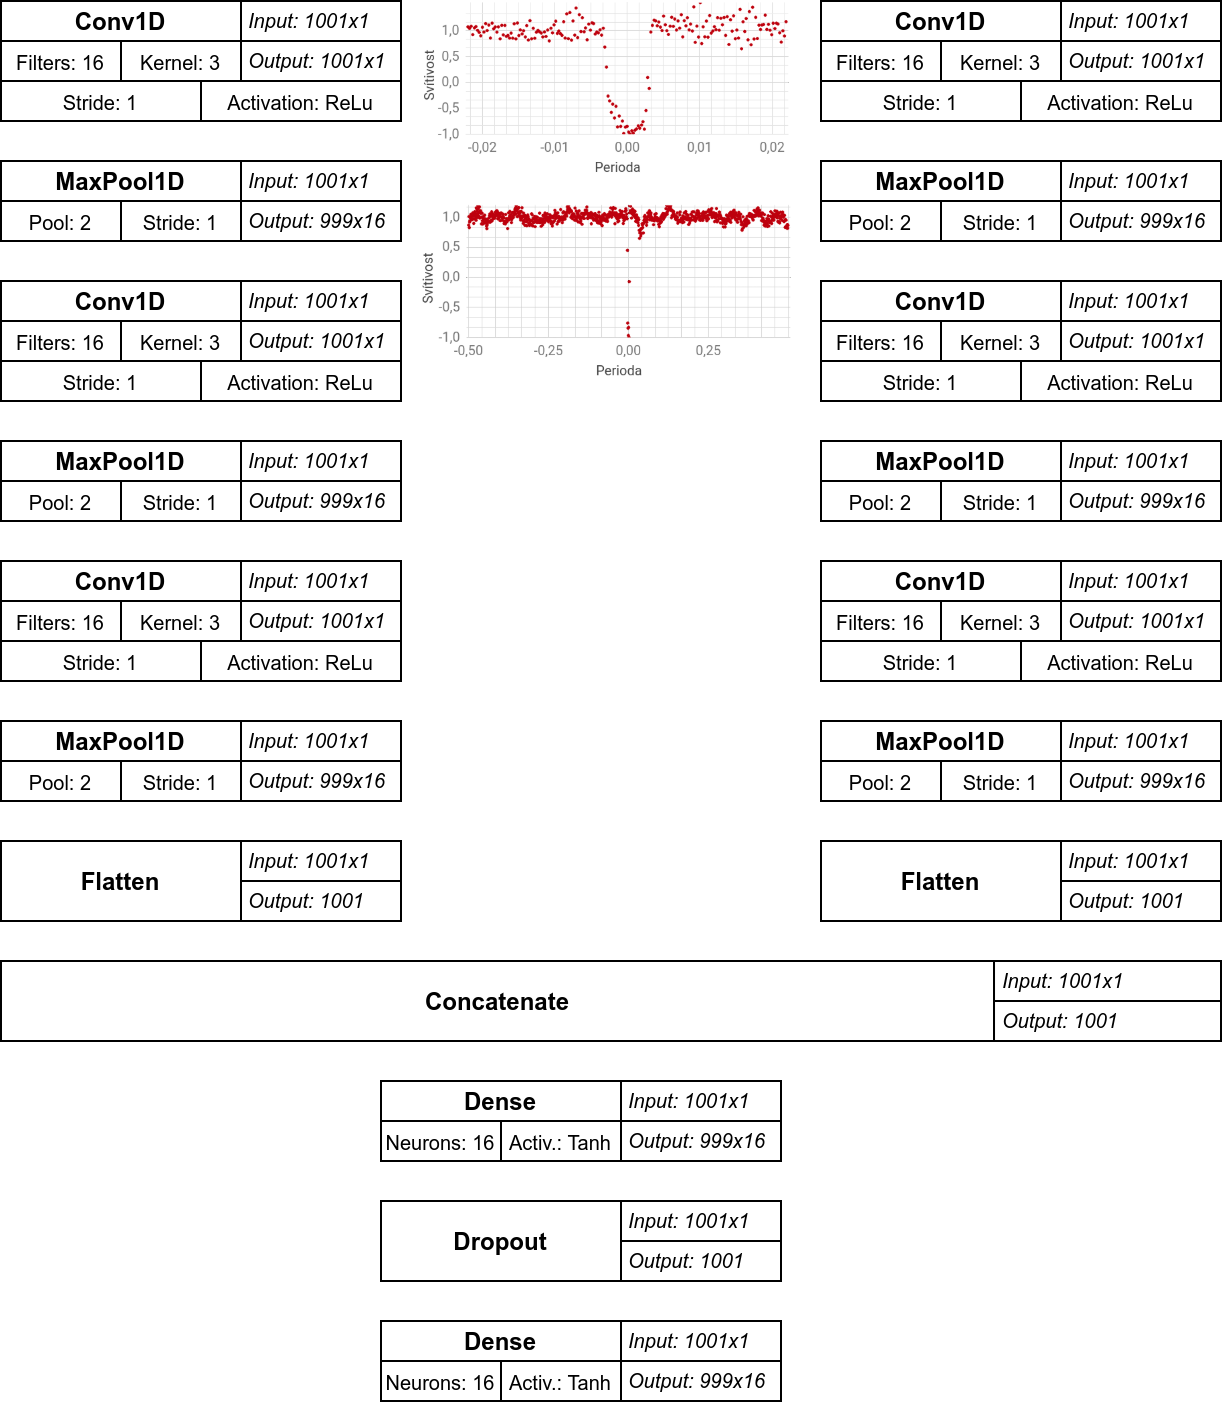
\includegraphics[width=\linewidth]{img/lc_cnn.png}

\section*{Příloha~B -- Architektura databáze}\label{priloha_b}
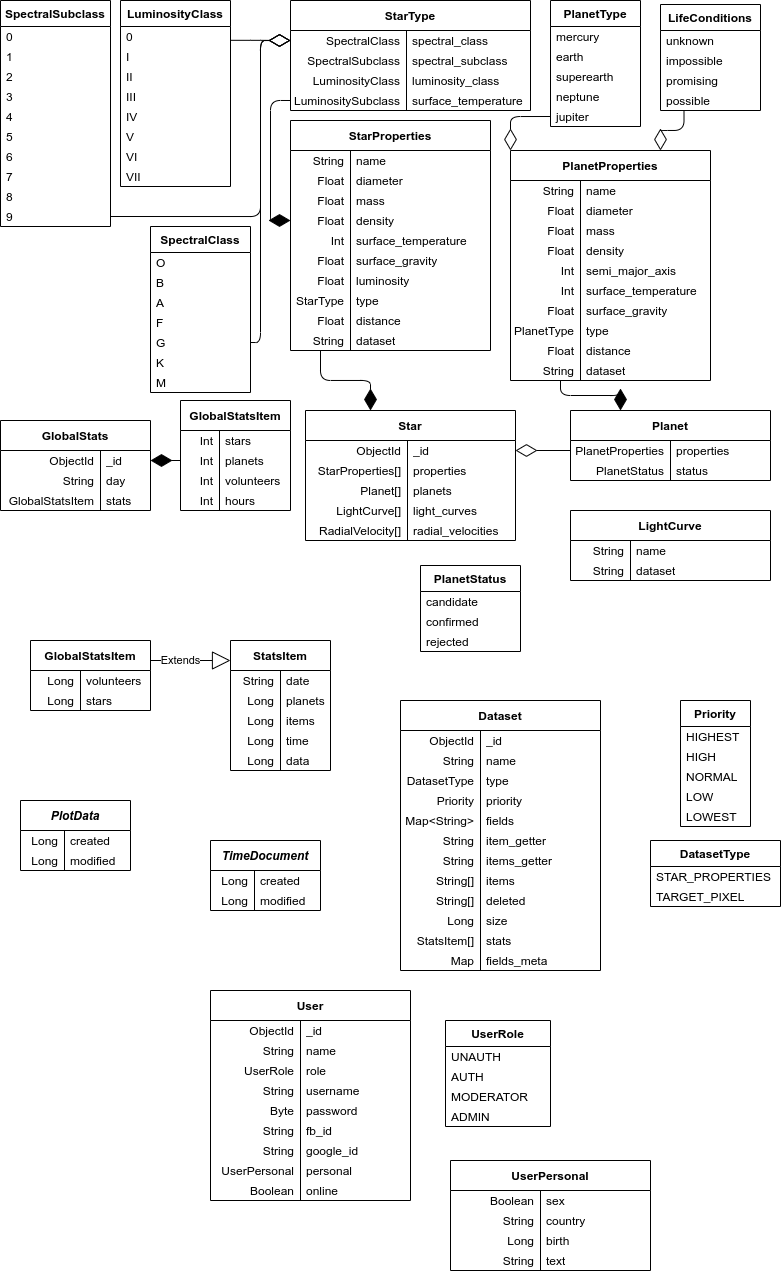
\includegraphics[width=\linewidth]{img/db.png}

\section*{Příloha~C -- Dokumentace REST API}\label{priloha_c}
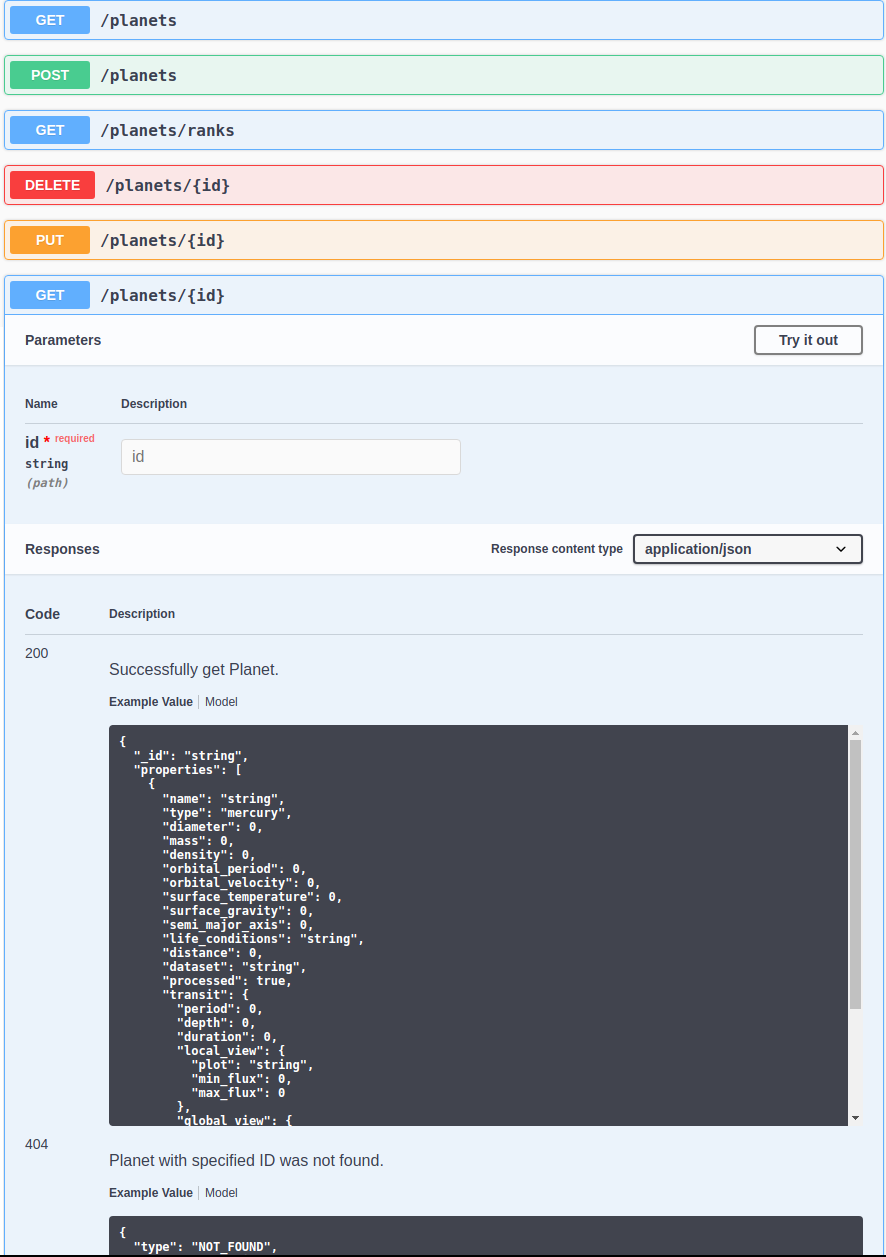
\includegraphics[width=\linewidth]{img/api_docs.png}

\section*{Příloha~D -- Verifikace výsledků}\label{priloha_d}
\begin{table}[!ht]
	\def\arraystretch{1.2}
	\setlength{\tabcolsep}{1pt}
	\begin{tabularx}{\textwidth}{|p{60pt}|X|X|X|X|X|X|X|X|X|X|X|X|}
		\hline
		\rowcolor{lightgray}
		\multicolumn{11}{|c|}{\textbf{Pozitivní}} \\
		\hline
		\rowcolor{lightgray}
		& & \multicolumn{3}{|l|}{Perioda oběhu [d]} & \multicolumn{3}{|l|}{Rov. poloměr [$r_\oplus$]} & \multicolumn{3}{|l|}{Hmotnost [$m_\oplus$]} \\	
		\hline	
		\rowcolor{lightgray}
		Planeta & Detekce & Vlastní & NASA & Chyba & Vlastní & NASA & Chyba & Vlastní & NASA & Chyba \\
		\hline	
		Kepler-39 b & \cellcolor{lightgreen} Ano & 21.087 & 21.087 & \cellcolor{lightgreen} 0 & 14.8 & 14.77 & \cellcolor{lightgreen} 0.0020 & 447 & 5688 & \cellcolor{lightred} 0.9214  \\	
		\hline	
		Kepler-40 b & \cellcolor{lightgreen} Ano & 6.873 & 6.873 & \cellcolor{lightgreen} 0 & 13.802 & 13.8 & \cellcolor{lightgreen} 0.0001 & 379.5 & 674 & \cellcolor{lightorange} 0.4369 \\	
		\hline	
		Kepler-41 b & \cellcolor{lightgreen} Ano & 1.856 & 1.856 & \cellcolor{lightgreen} 0 & 8.609 & 10.24 & \cellcolor{lightorange} 0.1593 & 136.9 & 174.8 & \cellcolor{lightorange} 0.2168 \\	
		\hline	
		Kepler-43 b & \cellcolor{lightgreen} Ano & 3.024 & 3.024 & \cellcolor{lightgreen} 0 & 12.21 & 12.5 & \cellcolor{lightgreen} 0.023 & 282.3 & 998 & \cellcolor{lightred} 0.7171 \\	
		\hline	
		Kepler-45 b & \cellcolor{lightgreen} Ano & 2.455 & 2.455 & \cellcolor{lightgreen} 0 & 10.853 & 11.03 & \cellcolor{lightgreen} 0.0163 & 212.17 & 150.5 & \cellcolor{lightorange} 0.4147 \\	
		\hline	
		Kepler-63 b & \cellcolor{lightgreen} Ano & 9.434 & 9.434 & \cellcolor{lightgreen} 0 & 5.64 & 6.11 & \cellcolor{lightgreen} 0.0777 & 203 & 120 & \cellcolor{lightred} 0.6917 \\	
		\hline	
		Kepler-66 b & \cellcolor{lightgreen} Ano & 17.816 & 17.816 & \cellcolor{lightgreen} 0 & 2.389 & 2.81 & \cellcolor{lightorange} 0.1498 & 14.16 & & \\
		\hline	
		Kepler-69 b & \cellcolor{lightgreen} Ano & 13.722 & 13.722 & \cellcolor{lightgreen} 0 & 2.165 & 2.28 & \cellcolor{lightgreen} 0.0504 & 10.43 &  & \\		
		\hline	
		Kepler-69 c & \cellcolor{lightred} Ne & & 242.467 & & & 1.74 & & & & \\	
		\hline	
		Kepler-74 b & \cellcolor{lightgreen} Ano & 7.341 & 7.341 & \cellcolor{lightgreen} 0 & 14.1 & 14.31 & \cellcolor{lightgreen} 0.014 & 396 & 216 & \cellcolor{lightred} 0.8333 \\	
		\hline	
		Kepler-75 b & \cellcolor{lightgreen} Ano & 8.887 & 8.887 & \cellcolor{lightgreen} 0 & 9.48 & 10.82 & \cellcolor{lightorange} 0.1238 & 167 & 3146 & \cellcolor{lightred} 0.9440 \\	
		\hline	
		Kepler-76 b & \cellcolor{lightgreen} Ano & 1.545 & 1.545 & \cellcolor{lightgreen} 0 & 9.74 & 13.67 & \cellcolor{lightorange} 0.2875 & 176 & 636 & \cellcolor{lightred} 0.7232 \\	
		\hline	
		Kepler-77 b & \cellcolor{lightgreen} Ano & 3.579 & 3.579 & \cellcolor{lightgreen} 0 & 10.719 & 10.761 & \cellcolor{lightgreen} 0.0039 & 206 & 225 & \cellcolor{lightgreen} 0.0844 \\	
		\hline	
		Kepler-78 b & \cellcolor{lightgreen} Ano & 0.355 & 0.355 & \cellcolor{lightgreen} 0 & 1.315 & 1.2 & \cellcolor{lightgreen} 0.0958 & 2.85 & 1.96 & \cellcolor{lightorange} 0.4541 \\	
		\hline	
		Kepler-79 b & \cellcolor{lightred} Ne & & 13.485 & & 3.47 & & & 10.9 & & \\	
		\hline	
		Kepler-79 c & \cellcolor{lightred} Ne & & 27.402 & & 3.72 & & & 12.5 & & \\	
		\hline	
		Kepler-79 d & \cellcolor{lightgreen} Ano & 52.09 & 52.09 & \cellcolor{lightgreen} 0 & 7.244 & 7.239 & \cellcolor{lightgreen} 0.0007 & 96.3 & & \\	
		\hline	
		Kepler-80 b & \cellcolor{lightgreen} Ano & 7.053 & 7.053 & \cellcolor{lightgreen} 0 & 2.07 & 2.21 & \cellcolor{lightgreen} 0.0676 & 9.1 & 6.94 & \cellcolor{lightorange} 0.3112 \\	
		\hline
		Kepler-91 b & \cellcolor{lightgreen} Ano & 6.25 & 6.25 & \cellcolor{lightgreen} 0 & 13.9 & 14.5 & \cellcolor{lightgreen} 0.0414 & 385 & 241 & \cellcolor{lightred} 0.5975 \\	
		\hline
		Kepler-95 b & \cellcolor{lightgreen} Ano & 11.523 & 11.523 & \cellcolor{lightgreen} 0 & 3.22 & 3.13 & \cellcolor{lightgreen} 0.0288 & 35.6 & & \\	
		\hline		
		Kepler-96 b & \cellcolor{lightgreen} Ano & 16.238 & 16.238 & \cellcolor{lightgreen} 0 & 2.55 & 2.55 & \cellcolor{lightgreen} 0 & 17.4 & 8.46 & \cellcolor{lightred} 1.0567 \\	
		\hline	
		Kepler-98 b & \cellcolor{lightgreen} Ano & 1.542 & 1.542 & \cellcolor{lightgreen} 0 & 1.59 & 1.82 & \cellcolor{lightorange} 0.1264 & 3.99 & 3.55 & \cellcolor{lightorange} 0.1103 \\	
		\hline
		Kepler-99 b & \cellcolor{lightgreen} Ano & 4.604 & 4.604 & \cellcolor{lightgreen} 0 & 1.48 & 1.48 & \cellcolor{lightgreen} 0 & 3.21 & 1.88 & \cellcolor{lightred} 0.7074 \\	
		\hline		
		Kepler-425 b & \cellcolor{lightgreen} Ano & 3.797 & 3.797 & \cellcolor{lightgreen} 0 & 9.48 & 9.84 & \cellcolor{lightgreen} 0.0366 & 167 & 79.45 & \cellcolor{lightred} 1.1019 \\	
		\hline	
		Kepler-426 b & \cellcolor{lightgreen} Ano & 3.218 & 3.218 & \cellcolor{lightgreen} 0 & 9.52 & 12.22 & \cellcolor{lightorange} 0.2209 & 169 & 108 & \cellcolor{lightred} 0.5648 \\	
		\hline	
	\end{tabularx}
\end{table}

\vspace{-20pt}

\begin{table}[!ht]
	\def\arraystretch{1.2}
	\setlength{\tabcolsep}{1pt}
	\begin{tabularx}{\textwidth}{|p{50pt}|X|p{50pt}|X|p{50pt}|X|p{50pt}|X|p{50pt}|X|p{50pt}|X|}
		\hline
		\rowcolor{lightgray}
		\multicolumn{10}{|c|}{\textbf{Negativní}} \\
		\hline
		\rowcolor{lightgray}
		KIC & Detekce & KIC & Detekce & KIC & Detekce & KIC & Detekce & KIC & Detekce \\	
		\hline
		100000925 & \cellcolor{lightgreen} Ne & 100000926 & \cellcolor{lightgreen} Ne & 100000927 & \cellcolor{lightgreen} Ne & 100000928 & \cellcolor{lightgreen} Ne & 100000929 & \cellcolor{lightgreen} Ne \\
		\hline
		100000930 & \cellcolor{lightgreen} Ne & 100000931 & \cellcolor{lightgreen} Ne & 100000932 & \cellcolor{lightgreen} Ne & 100000933 & \cellcolor{lightgreen} Ne & 100000934 & \cellcolor{lightgreen} Ne \\
		\hline
		100000935 & \cellcolor{lightgreen} Ne & 100000936 & \cellcolor{lightgreen} Ne & 100000937 & \cellcolor{lightgreen} Ne & 100000938 & \cellcolor{lightgreen} Ne & 100000939 & \cellcolor{lightgreen} Ne \\
		\hline
		100000940 & \cellcolor{lightgreen} Ne & 100000941 & \cellcolor{lightgreen} Ne & 100000942 & \cellcolor{lightgreen} Ne & 100000943 & \cellcolor{lightgreen} Ne & 100000944 & \cellcolor{lightgreen} Ne \\
		\hline
		100000945 & \cellcolor{lightgreen} Ne & 100000946 & \cellcolor{lightgreen} Ne & 100000947 & \cellcolor{lightgreen} Ne & 100000948 & \cellcolor{lightgreen} Ne & 100000949 & \cellcolor{lightgreen} Ne \\
		\hline
		100000950 & \cellcolor{lightgreen} Ne & 100000951 & \cellcolor{lightgreen} Ne & 100000952 & \cellcolor{lightgreen} Ne & 100000953 & \cellcolor{lightgreen} Ne & 100000954 & \cellcolor{lightgreen} Ne \\
		\hline
		100000955 & \cellcolor{lightgreen} Ne & 100000956 & \cellcolor{lightgreen} Ne & 100000957 & \cellcolor{lightgreen} Ne & 100000958 & \cellcolor{lightgreen} Ne & 100000959 & \cellcolor{lightgreen} Ne \\
		\hline
		100000960 & \cellcolor{lightgreen} Ne & 100000961 & \cellcolor{lightgreen} Ne & 100000962 & \cellcolor{lightgreen} Ne & 100000963 & \cellcolor{lightgreen} Ne & 100000964 & \cellcolor{lightgreen} Ne \\
		\hline
		4928826 & \cellcolor{lightgreen} Ne & 4928862 & \cellcolor{lightgreen} Ne & 4928898 & \cellcolor{lightgreen} Ne & 4932320 & \cellcolor{lightgreen} Ne & 4936238 & \cellcolor{lightgreen} Ne \\
		\hline
		4936281 & \cellcolor{lightgreen} Ne & 4936287 & \cellcolor{lightgreen} Ne & 4940980 & \cellcolor{lightgreen} Ne & 4940999 & \cellcolor{lightgreen} Ne & 4941156 & \cellcolor{lightgreen} Ne \\
		\hline
		4929214 & \cellcolor{lightgreen} Ne & 4929259 & \cellcolor{lightgreen} Ne & 4929301 & \cellcolor{lightgreen} Ne & 4929426 & \cellcolor{lightgreen} Ne & 4929449 & \cellcolor{lightgreen} Ne \\
		\hline
		8396995 & \cellcolor{lightgreen} Ne & 8397017 & \cellcolor{lightgreen} Ne & 8397026 & \cellcolor{lightgreen} Ne & 8397068 & \cellcolor{lightgreen} Ne & 8397111 & \cellcolor{lightgreen} Ne \\
		\hline
	\end{tabularx}
\end{table}
\end{document}